\chapter{Testing and Evaluation Process}
\label{chap:testing_process}

This section details the comprehensive testing and evaluation process designed to ensure the Library Management System (LMS) meets the specified requirements and quality standards. Our strategy employs a multi-layered approach, combining static and dynamic testing techniques across various levels of the application architecture. The process is structured to systematically identify, document, and resolve defects throughout the software development lifecycle (SDLC).

The primary objectives of our testing process are to:
\begin{itemize}
    \item Verify that all functional requirements outlined in the Software Requirements Specification (SRS) are correctly implemented.
    \item Ensure that the system meets all non-functional requirements, including performance, security, and usability benchmarks.
    \item Validate the system's stability, reliability, and robustness through rigorous integration, regression, and end-to-end testing.
    \item Provide comprehensive test coverage reports and defect analyses to stakeholders for informed decision-making.
\end{itemize}

\section{Testing Strategy Overview}
Our testing strategy is built upon a foundation of continuous testing, integrating quality assurance activities into every phase of the development cycle. The strategy is visualized in Figure \ref{fig:testing_process_flow}. It begins with static testing techniques like code and documentation reviews, followed by a hierarchy of dynamic testing levels, from unit testing of individual components to system-wide end-to-end testing.

\begin{figure}[H]
    \centering
    \resizebox{0.7\textwidth}{!}{%
        \begin{tikzpicture}[
            node distance=1.5cm and 2cm,
            block/.style={rectangle, draw, fill=blue!10, text width=8em, text centered, rounded corners, minimum height=3em, drop shadow},
            line/.style={draw, -{Stealth[length=3mm, width=2mm]}},
            cloud/.style={ellipse, draw, fill=gray!10, text width=6em, text centered, minimum height=3em, drop shadow}
        ]
            % Nodes
                        \node[cloud] (srs) {SRS \& Requirements};
                        \node[block, below=of srs] (planning) {Test Planning \& Design};
                        \node[block, below left=of planning, xshift=0cm] (static) {Static Testing};
                        \node[block, below right=of planning, xshift=-2cm] (dynamic) {Dynamic Testing};
                        
                        % Static Testing Branch
                        \node[block, below=of static, text width=9em] (review) {Code \& Document Reviews};
                        
                        % Dynamic Testing Branch
                        \node[block, below=of dynamic] (unit) {Unit Testing (Jest)};
                        \node[block, below=of unit] (integration) {API \& Integration Testing (Jest/Supertest)};
                        \node[block, below=of integration] (system) {System E2E Testing (Cypress)};
                        \node[block, below=of system] (non-func) {Non-Functional Testing};
                        
                        % Merge back
                        \node[block, below=of planning, yshift=-10cm, xshift=-2cm] (regression) {Regression Testing};
                        \node[block, below=of regression] (defect) {Defect Management};
                        \node[block, below=of defect] (report) {Reporting \& Sign-off};

                        % Paths
                        \path[line] (srs) -- (planning);
                        \path[line] (planning) -- (static);
                        \path[line] (planning) -- (dynamic);
                        \path[line] (static) -- (review);
                        \path[line] (dynamic) -- (unit);
                        \path[line] (unit) -- (integration);
                        \path[line] (integration) -- (system);
                        \path[line] (system) -- (non-func);
                        
                        % Converge paths to regression
                        \path[line] (review) |- (regression);
                        \path[line] (non-func.west) -- (regression.east);
                        
                        \path[line] (regression) -- (defect);
                        \path[line] (defect) -- (report);
        \end{tikzpicture}%
    }
    \caption{Overall Testing Process Flowchart}
    \label{fig:testing_process_flow}
\end{figure}

\section{Testing Levels}
Testing is structured into distinct levels to ensure all parts of the system are validated, from the smallest code unit to the fully integrated application.

\subsection{Unit Testing}
Unit tests focus on the smallest individual components of the application in isolation. This is primarily aimed at the controllers, models, and utility functions within the Node.js backend.
\begin{itemize}
    \item \textbf{Objective:} To verify that each function or module behaves as expected.
    \item \textbf{Framework:} Jest is used as the testing framework, assertion library, and test runner.
    \item \textbf{Methodology:} Dependencies such as database models or external services are mocked to ensure tests are fast, reliable, and isolated. Test cases cover both successful paths and error conditions.
\end{itemize}
Detailed unit test cases are documented in the corresponding test file.
\subsubsection{Authentication Controller (authController)}

The Auth Controller is responsible for user authentication, including registration (by a librarian), login, and logout. These tests ensure that access control and user session management are functioning correctly, as specified in the SRS.

\begin{longtable}{|p{0.1\textwidth}|p{0.15\textwidth}|p{0.15\textwidth}|p{0.20\textwidth}|p{0.25\textwidth}|}
    \caption{Test Cases for authController}\\
    \hline
    \textbf{Test Case ID} & \textbf{Related Requirement (SRS)} & \textbf{Test Scenario} & \textbf{Test Steps} & \textbf{Expected Result} \\
    \hline
    \endfirsthead
    \multicolumn{5}{c}%
    {{\bfseries \tablename\ \thetable{} -- continued from previous page}} \\
    \hline
    \textbf{Test Case ID} & \textbf{Related Requirement (SRS)} & \textbf{Test Scenario} & \textbf{Test Steps} & \textbf{Expected Result} \\
    \hline
    \endhead
    \hline \multicolumn{5}{|r|}{{Continued on next page}} \\ \hline
    \endfoot
    \hline
    \endlastfoot

    % Test Cases for registerUser
    TC-AUTH-001 & 3.1.1 User Registration , UC-004  & Successful user registration & 1. Mock \texttt{User.findOne} to resolve as null. \newline 2. Mock \texttt{User.create} to resolve with a new user object. \newline 3. Call \texttt{registerUser} with valid new user data. & 1. Response status is 201. \newline 2. Response JSON indicates successful registration. \\
    \hline
    TC-AUTH-002 & UC-004 (A1: Email Already Exists)  & Attempt to register a user that already exists & 1. Mock \texttt{User.findOne} to resolve with an existing user object. \newline 2. Call \texttt{registerUser} with data of an existing user. & 1. Response status is 400. \newline 2. Response JSON indicates that the username or email already exists. \\
    \hline

    % Test Cases for loginUser
    TC-AUTH-003 & 3.1.2 User Login , UC-001  & Successful user login with valid credentials & 1. Mock \texttt{passport.authenticate} to succeed and return a user object. \newline 2. Call \texttt{loginUser} middleware with correct username and password. & 1. \texttt{req.logIn} is called. \newline 2. Response status is 200. \newline 3. Response JSON indicates successful login and includes user data. \\
    \hline
    TC-AUTH-004 & UC-001 (A1: Invalid Credentials)  & Attempt to login with invalid credentials & 1. Mock \texttt{passport.authenticate} to fail (returns false). \newline 2. Call \texttt{loginUser} middleware with an incorrect username or password. & 1. Response status is 401. \newline 2. Response JSON indicates incorrect credentials. \\
    \hline

    % Test Cases for logoutUser
    TC-AUTH-005 & 3.1.3 User Logout  & Successful user logout & 1. Mock \texttt{req.logout}. \newline 2. Call \texttt{logoutUser}. & 1. \texttt{req.logout} is called. \newline 2. Response status is 200. \newline 3. Response JSON indicates successful logout. \\
    \hline
\end{longtable}

\subsubsection{Author Controller (authorController)}


The Author Controller manages CRUD operations for author entities. These tests validate the creation and retrieval of authors.

\begin{longtable}{|p{0.1\textwidth}|p{0.2\textwidth}|p{0.2\textwidth}|p{0.25\textwidth}|p{0.25\textwidth}|}
    \caption{Test Cases for authorController}\\
    \hline
    \textbf{Test Case ID} & \textbf{Related Requirement (SRS)} & \textbf{Test Scenario} & \textbf{Test Steps} & \textbf{Expected Result} \\
    \hline
    \endfirsthead
    \multicolumn{5}{c}%
    {{\bfseries \tablename\ \thetable{} -- continued from previous page}} \\
    \hline
    \textbf{Test Case ID} & \textbf{Related Requirement (SRS)} & \textbf{Test Scenario} & \textbf{Test Steps} & \textbf{Expected Result} \\
    \hline
    \endhead
    \hline \multicolumn{5}{|r|}{{Continued on next page}} \\ \hline
    \endfoot
    \hline
    \endlastfoot

    % Test Cases for createAuthor
    TC-ATHR-001 & 3.4 Author Management (POST /api/author/add)  & Successfully create a new author & 1. Provide author details in \texttt{req.body}. \newline 2. Mock \texttt{Author.create} to resolve with the new author data. \newline 3. Call \texttt{createAuthor}. & 1. Response status is 201. \newline 2. Response JSON contains the newly created author. \\
    \hline

    % Test Cases for getAllAuthors
    TC-ATHR-002 & 3.4 Author Management (GET /api/author/getAll)  & Successfully retrieve all authors & 1. Mock \texttt{Author.find} to resolve with an array of author objects. \newline 2. Call \texttt{getAllAuthors}. & 1. Response status is 200. \newline 2. Response JSON contains the array of all authors. \\
    \hline
\end{longtable}

\subsubsection{Book Controller (bookController)}

The Book Controller handles all CRUD operations for book entities. The tests ensure that books can be created, retrieved (all and by ID), updated, and deleted as per the requirements.

\begin{longtable}{|p{0.1\textwidth}|p{0.2\textwidth}|p{0.2\textwidth}|p{0.25\textwidth}|p{0.25\textwidth}|}
    \caption{Test Cases for bookController}\\
    \hline
    \textbf{Test Case ID} & \textbf{Related Requirement (SRS)} & \textbf{Test Scenario} & \textbf{Test Steps} & \textbf{Expected Result} \\
    \hline
    \endfirsthead
    \multicolumn{5}{c}%
    {{\bfseries \tablename\ \thetable{} -- continued from previous page}} \\
    \hline
    \textbf{Test Case ID} & \textbf{Related Requirement (SRS)} & \textbf{Test Scenario} & \textbf{Test Steps} & \textbf{Expected Result} \\
    \hline
    \endhead
    \hline \multicolumn{5}{|r|}{{Continued on next page}} \\ \hline
    \endfoot
    \hline
    \endlastfoot

    % Test Cases
    TC-BOOK-001 & 3.3 Book Management (POST /api/book/add) , UC-002  & Successfully create a new book & 1. Provide book details in \texttt{req.body}. \newline 2. Mock \texttt{Book.create} to resolve successfully. \newline 3. Call \texttt{createBook}. & 1. Response status is 201. \newline 2. Response JSON contains the new book. \\
    \hline
    TC-BOOK-002 & UC-002 (A2: API Error)  & Fail to create a book due to a database error & 1. Mock \texttt{Book.create} to reject with an error. \newline 2. Call \texttt{createBook}. & 1. Response status is 500. \newline 2. Response JSON contains an error message. \\
    \hline
    TC-BOOK-003 & 3.3 Book Management (GET /api/book/getAll)  & Successfully retrieve all books & 1. Mock \texttt{Book.find().populate()} to resolve with an array of books. \newline 2. Call \texttt{getAllBooks}. & 1. Response status is 200. \newline 2. Response JSON contains the array of books. \\
    \hline
    TC-BOOK-004 & 3.3 Book Management (GET /api/book/get/:id)  & Successfully retrieve a single book by its ID & 1. Provide a book ID in \texttt{req.params}. \newline 2. Mock \texttt{Book.findById().populate()} to resolve with a book object. \newline 3. Call \texttt{getBookById}. & 1. Response status is 200. \newline 2. Response JSON contains the specific book. \\
    \hline
    TC-BOOK-005 & 3.3 Book Management (GET /api/book/get/:id)  & Attempt to retrieve a book with a non-existent ID & 1. Provide a non-existent book ID in \texttt{req.params}. \newline 2. Mock \texttt{Book.findById().populate()} to resolve as null. \newline 3. Call \texttt{getBookById}. & 1. Response status is 404. \newline 2. Response JSON contains a 'Book not found' message. \\
    \hline
    TC-BOOK-006 & 3.3 Book Management (PUT /api/book/update/:id) & Successfully update an existing book & 1. Provide a book ID and update data. \newline 2. Mock \texttt{Book.findByIdAndUpdate} to resolve with the updated book. \newline 3. Call \texttt{updateBook}. & 1. Response status is 200. \newline 2. Response JSON contains the updated book data. \\
    \hline
    TC-BOOK-007 & 3.3 Book Management (DELETE /api/book/delete/:id)  & Successfully delete a book & 1. Provide a book ID to be deleted. \newline 2. Mock \texttt{Book.findByIdAndDelete} to resolve successfully. \newline 3. Call \texttt{deleteBook}. & 1. Response status is 200. \newline 2. Response JSON contains a 'Book removed' message. \\
    \hline
\end{longtable}

\subsubsection{Borrowal Controller (borrowalController)}

This controller manages borrowal records. Tests cover creating a borrowal (and updating book availability), updating a borrowal's status, and retrieving borrowals based on user roles (Librarian vs. Member).

\begin{longtable}{|p{0.1\textwidth}|p{0.2\textwidth}|p{0.2\textwidth}|p{0.25\textwidth}|p{0.25\textwidth}|}
    \caption{Test Cases for borrowalController}\\
    \hline
    \textbf{Test Case ID} & \textbf{Related Requirement (SRS)} & \textbf{Test Scenario} & \textbf{Test Steps} & \textbf{Expected Result} \\
    \hline
    \endfirsthead
    \multicolumn{5}{c}%
    {{\bfseries \tablename\ \thetable{} -- continued from previous page}} \\
    \hline
    \textbf{Test Case ID} & \textbf{Related Requirement (SRS)} & \textbf{Test Scenario} & \textbf{Test Steps} & \textbf{Expected Result} \\
    \hline
    \endhead
    \hline \multicolumn{5}{|r|}{{Continued on next page}} \\ \hline
    \endfoot
    \hline
    \endlastfoot

    % Test Cases
    TC-BORR-001 & 3.6 Borrowal Management , UC-003  & Create a borrowal for an available book & 1. Mock \texttt{Book.findById} to return an available book. \newline 2. Mock \texttt{Borrowal.create} to succeed. \newline 3. Call \texttt{createBorrowal}. & 1. Book's availability is set to false. \newline 2. Response status is 201. \newline 3. Response JSON contains the new borrowal record. \\
    \hline
    TC-BORR-002 & UC-003 (A1: Book Not Available)  & Attempt to create a borrowal for an unavailable book & 1. Mock \texttt{Book.findById} to return an unavailable book. \newline 2. Call \texttt{createBorrowal}. & 1. Response status is 400. \newline 2. Response JSON has a "Book is not available" message. \\
    \hline
    TC-BORR-003 & 3.6 Borrowal Management (PUT /api/borrowal/update/:id)  & Update borrowal status to 'Returned' & 1. Mock \texttt{Borrowal.findById} to find a borrowal. \newline 2. Mock \texttt{Book.findByIdAndUpdate} to succeed. \newline 3. Call \texttt{updateBorrowal} with status 'Returned'. & 1. Book's availability is set to true. \newline 2. Response status is 200. \newline 3. Response JSON contains the updated borrowal. \\
    \hline
    TC-BORR-004 & 3.6 Borrowal Management (GET /api/borrowal/getAll)  & Get all borrowals as a Librarian & 1. Set \texttt{req.user.role} to 'Librarian'. \newline 2. Mock \texttt{Borrowal.find} to return all borrowals. \newline 3. Call \texttt{getBorrowals}. & 1. \texttt{Borrowal.find} is called with an empty filter. \newline 2. Response contains all borrowal records. \\
    \hline
    TC-BORR-005 & 3.6 Borrowal Management , UC-005  & Get own borrowals as a Member & 1. Set \texttt{req.user.role} to 'Member'. \newline 2. Mock \texttt{Borrowal.find} to return member-specific borrowals. \newline 3. Call \texttt{getBorrowals}. & 1. \texttt{Borrowal.find} is called with a filter for the member's ID. \newline 2. Response contains only the member's borrowals. \\
    \hline
\end{longtable}

\subsubsection{Genre Controller (genreController)}

The Genre Controller manages CRUD operations for genre entities. These tests validate the creation and retrieval of genres.

\begin{longtable}{|p{0.1\textwidth}|p{0.2\textwidth}|p{0.2\textwidth}|p{0.25\textwidth}|p{0.25\textwidth}|}
    \caption{Test Cases for genreController}\\
    \hline
    \textbf{Test Case ID} & \textbf{Related Requirement (SRS)} & \textbf{Test Scenario} & \textbf{Test Steps} & \textbf{Expected Result} \\
    \hline
    \endfirsthead
    \multicolumn{5}{c}%
    {{\bfseries \tablename\ \thetable{} -- continued from previous page}} \\
    \hline
    \textbf{Test Case ID} & \textbf{Related Requirement (SRS)} & \textbf{Test Scenario} & \textbf{Test Steps} & \textbf{Expected Result} \\
    \hline
    \endhead
    \hline \multicolumn{5}{|r|}{{Continued on next page}} \\ \hline
    \endfoot
    \hline
    \endlastfoot

    % Test Cases for createGenre
    TC-GENR-001 & 3.5 Genre Management (POST /api/genre/add)  & Successfully create a new genre & 1. Provide genre details in \texttt{req.body}. \newline 2. Mock \texttt{Genre.create} to resolve with the new genre data. \newline 3. Call \texttt{createGenre}. & 1. Response status is 201. \newline 2. Response JSON contains the newly created genre. \\
    \hline

    % Test Cases for getAllGenres
    TC-GENR-002 & 3.5 Genre Management (GET /api/genre/getAll)  & Successfully retrieve all genres & 1. Mock \texttt{Genre.find} to resolve with an array of genre objects. \newline 2. Call \texttt{getAllGenres}. & 1. Response status is 200. \newline 2. Response JSON contains the array of all genres. \\
    \hline
\end{longtable}

\subsubsection{Review Controller (reviewController)}

The Review Controller is responsible for managing book reviews. The tests cover the creation of reviews and fetching all reviews for a specific book.

\begin{longtable}{|p{0.1\textwidth}|p{0.2\textwidth}|p{0.2\textwidth}|p{0.25\textwidth}|p{0.25\textwidth}|}
    \caption{Test Cases for reviewController}\\
    \hline
    \textbf{Test Case ID} & \textbf{Related Requirement (SRS)} & \textbf{Test Scenario} & \textbf{Test Steps} & \textbf{Expected Result} \\
    \hline
    \endfirsthead
    \multicolumn{5}{c}%
    {{\bfseries \tablename\ \thetable{} -- continued from previous page}} \\
    \hline
    \textbf{Test Case ID} & \textbf{Related Requirement (SRS)} & \textbf{Test Scenario} & \textbf{Test Steps} & \textbf{Expected Result} \\
    \hline
    \endhead
    \hline \multicolumn{5}{|r|}{{Continued on next page}} \\ \hline
    \endfoot
    \hline
    \endlastfoot

    % Test Cases for createReview
    TC-REV-001 & 3.8 Review Management (POST /api/review/add)  & Successfully create a review for a book & 1. Provide review details (bookId, rating, comment) in \texttt{req.body}. \newline 2. Mock \texttt{Review.create} to resolve with the new review object. \newline 3. Call \texttt{createReview}. & 1. Response status is 201. \newline 2. Response JSON contains the newly created review. \\
    \hline

    % Test Cases for getReviewsForBook
    TC-REV-002 & 3.8 Review Management  & Get all reviews for a specific book & 1. Provide a book ID in \texttt{req.params.bookId}. \newline 2. Mock \texttt{Review.find().populate()} to resolve with an array of reviews. \newline 3. Call \texttt{getReviewsForBook}. & 1. \texttt{Review.find} is called with a filter for the book ID. \newline 2. Response status is 200. \newline 3. Response JSON contains the array of reviews for that book. \\
    \hline
\end{longtable}

\subsection{Integration Testing}
Integration testing focuses on verifying the interaction between different components. For the LMS, this primarily involves testing the API endpoints to ensure they correctly interact with controllers, models, and the database.
\begin{itemize}
    \item \textbf{Objective:} To detect defects in the interfaces and interactions between integrated components.
    \item \textbf{Framework:} Jest and Supertest are used to send HTTP requests to the API endpoints and assert the responses.
    \item \textbf{Methodology:} Tests cover creating, reading, updating, and deleting (CRUD) entities, as well as complex workflows involving multiple API calls. A test database is used to ensure a clean state for each test run.
\end{itemize}
The specific test cases for integration testing are detailed in:
\begin{longtable}{|>{\scriptsize\raggedright\arraybackslash}p{3cm}|>{\raggedright\arraybackslash}p{4cm}|>{\raggedright\arraybackslash}p{5.5cm}|>{\raggedright\arraybackslash}p{5.5cm}|}
\caption{Integration Test Cases}\label{tab:integration_test_cases}\\
\hline
\textbf{Test Case ID} & \textbf{Test Title / Scenario} & \textbf{Test Steps} & \textbf{Expected Results} \\
\hline
\endfirsthead
\multicolumn{4}{c}%
{{\bfseries \tablename\ \thetable{} -- continued from previous page}} \\
\hline
\textbf{Test Case ID} & \textbf{Test Title / Scenario} & \textbf{Test Steps} & \textbf{Expected Results} \\
\hline
\endhead
\hline \multicolumn{4}{|r|}{{Continued on next page}} \\ \hline
\endfoot
\hline
\endlastfoot

% Scenario 1: Full Book and User Lifecycle
\multicolumn{4}{|l|}{\textbf{Scenario: Full Lifecycle - From Entity Creation to Borrowal}} \\ \hline
TC\_INT\_001 & End-to-end workflow of creating all required entities for a new book, registering a new member, and the member borrowing that book. & 
    \begin{itemize}[noitemsep, topsep=0pt, partopsep=0pt, leftmargin=*]
        \item \textbf{As Librarian:} Login to the system.
        \item Navigate to Author Management and add a new author (e.g., "J.R.R. Tolkien").
        \item Navigate to Genre Management and add a new genre (e.g., "Fantasy").
        \item Navigate to Book Management and add a new book ("The Hobbit"), linking the newly created author and genre. Set `isAvailable` to true.
        \item Navigate to User Management and register a new user with `isAdmin=false` (e.g., "Member1").
        \item Logout.
        \item \textbf{As Member1:} Login to the system.
        \item Navigate to the book list and find "The Hobbit".
        \item Initiate and confirm the borrowing of "The Hobbit".
    \end{itemize} & 
    \begin{itemize}[noitemsep, topsep=0pt, partopsep=0pt, leftmargin=*]
        \item The author is created successfully and selectable in the book form.
        \item The genre is created successfully and selectable in the book form.
        \item The book is created with correct author and genre associations. The book list shows its status as available.
        \item The new member account is created and appears in the user list.
        \item Member1 can log in successfully and is directed to the member landing page.
        \item A new borrowal record is created for Member1 and "The Hobbit".
        \item The `isAvailable` status of "The Hobbit" in the Book entity is updated to `false`.
        \item The new borrowal record appears in Member1's borrowal history.
    \end{itemize} \\ \hline

% Scenario 2: Data Integrity on Deletion
\multicolumn{4}{|l|}{\textbf{Scenario: Data Integrity and Referential Constraints}} \\ \hline
TC\_INT\_002 & Verify data integrity when a linked entity (Author) is deleted after being associated with another entity (Book). & 
    \begin{itemize}[noitemsep, topsep=0pt, partopsep=0pt, leftmargin=*]
        \item \textbf{As Librarian:} Login.
        \item Create a new, unique Author (e.g., "IntegTest Author").
        \item Create a new Book (e.g., "IntegTest Book") and link it to "IntegTest Author".
        \item Verify the book details page shows "IntegTest Author" as the author.
        \item Navigate to Author Management and delete "IntegTest Author".
        \item Navigate back to Book Management and view the details of "IntegTest Book".
    \end{itemize} & 
    \begin{itemize}[noitemsep, topsep=0pt, partopsep=0pt, leftmargin=*]
        \item The Author is successfully deleted.
        \item The Book "IntegTest Book" still exists in the system.
        \item The `authorId` field for "IntegTest Book" is handled gracefully (e.g., set to null or an empty value), as the data model indicates it's optional. The book details page no longer displays the deleted author's name.
        \item The system does not crash and remains in a consistent state.
    \end{itemize} \\ \hline
TC\_INT\_003 & Verify that deleting a User with active Borrowals does not violate data consistency. &
    \begin{itemize}[noitemsep, topsep=0pt, partopsep=0pt, leftmargin=*]
        \item \textbf{As Librarian:} Login.
        \item Ensure a specific Member (e.g., "MemberToDelete") has at least one active borrowal record. If not, create one.
        \item Navigate to User Management.
        \item Attempt to delete the user "MemberToDelete".
    \end{itemize} & 
    \begin{itemize}[noitemsep, topsep=0pt, partopsep=0pt, leftmargin=*]
        \item \textbf{Expected (Option A - Deletion Blocked):} The system prevents the deletion and displays an error message indicating the user has active borrowals that must be resolved first.
        \item \textbf{Expected (Option B - Soft Delete/Orphaning):} The user is deleted. The `memberId` in the Borrowal record  remains but now points to a non-existent user. The borrowal record is still visible to the Librarian, but may indicate the user is deleted.
        \item (The exact expected result depends on the implemented business rule for referential integrity, which should be consistent).
    \end{itemize} \\ \hline

% Scenario 3: State Transition
\multicolumn{4}{|l|}{\textbf{Scenario: State Transitions Across Modules}} \\ \hline
TC\_INT\_004 & Verify that the state of a Book (isAvailable) is correctly updated by actions in the Borrowal module. & 
    \begin{itemize}[noitemsep, topsep=0pt, partopsep=0pt, leftmargin=*]
        \item \textbf{Prerequisite:} A book "StateTest Book" exists and is available. A "StateTest Member" exists.
        \item \textbf{As Member:} Login as "StateTest Member". Borrow "StateTest Book".
        \item \textbf{As Librarian:} Login. Navigate to Book Management. View the status of "StateTest Book".
        \item Try to create a new borrowal for "StateTest Book" for another member.
        \item Navigate to Borrowal Management. Find the borrowal record for "StateTest Book" and update its status to "Returned".
        \item Navigate back to Book Management and view the status of "StateTest Book" again.
    \end{itemize} & 
    \begin{itemize}[noitemsep, topsep=0pt, partopsep=0pt, leftmargin=*]
        \item After the member borrows the book, the book's `isAvailable` status immediately changes to `false`.
        \item The Librarian cannot create a new borrowal for the now-unavailable book. The UI should prevent this action.
        \item After the Librarian marks the borrowal as "Returned", the borrowal record's status field is updated.
        \item The `isAvailable` status of "StateTest Book" in the Book module reverts to `true`.
        \item The data remains consistent between the Book and Borrowal modules throughout the workflow.
    \end{itemize} \\ \hline

% Scenario 4: Role-Based Access Control
\multicolumn{4}{|l|}{\textbf{Scenario: Role-Based Access Control (RBAC) Integration}} \\ \hline
TC\_INT\_005 & Verify that user roles created in the User module correctly restrict access to features in other modules (e.g., Book, Author). &
    \begin{itemize}[noitemsep, topsep=0pt, partopsep=0pt, leftmargin=*]
        \item \textbf{As Librarian:} Login. Create a new user "TestMember" with the role of Member (`isAdmin=false`).
        \item Logout.
        \item \textbf{As Member:} Login as "TestMember".
        \item Attempt to access the User Management page via direct URL navigation (e.g., `/users`).
        \item Navigate to the Books list.
        \item Check for the presence of "Add New Book", "Edit", or "Delete" buttons/options.
        \item Using an API client (e.g., Postman), attempt to send a `POST` request to `/api/book/add` using the session/token of "TestMember".
    \end{itemize} & 
    \begin{itemize}[noitemsep, topsep=0pt, partopsep=0pt, leftmargin=*]
        \item The Member login is successful.
        \item Direct navigation to the `/users` URL is blocked, and the user is redirected to the member dashboard or an error page.
        \item The UI for the Books list does not show any administrative controls (Add, Edit, Delete).
        \item The API request to `POST /api/book/add` fails with an authorization error (e.g., 403 Forbidden or 401 Unauthorized), demonstrating that the access control middleware correctly uses the user's role from the session.
    \end{itemize} \\ \hline

\end{longtable}

\subsection{System Testing}
System testing evaluates the complete and fully integrated application from an end-to-end (E2E) perspective. This level of testing simulates real user scenarios to validate the system against the requirements defined in the SRS.
\begin{itemize}
    \item \textbf{Objective:} To validate the complete system's compliance with its specified requirements.
    \item \textbf{Framework:} Cypress is used for E2E testing, automating user interactions in a real browser environment.
    \item \textbf{Methodology:} Test scripts simulate user workflows such as logging in, searching for a book, borrowing a book, and managing user accounts. Assertions are made on the UI to confirm that the application behaves as expected.
\end{itemize}


\section{Dynamic Testing Types}
Dynamic testing is performed while the code is executing. We have categorized our dynamic tests into functional and non-functional types to ensure comprehensive coverage.

\subsection{Functional Testing}
Functional testing verifies that the system performs its functions as specified in the SRS. Test cases are derived directly from the user stories and functional requirements.
\subsubsection{Authentication and Authorization}
\documentclass[10pt, a4paper]{report}
\usepackage[utf8]{inputenc}
\usepackage{geometry}
\usepackage{longtable}
\usepackage{array} % For better column definitions in longtable
\usepackage{enumitem} % Required for itemize and enumerate options
\usepackage{helvet} % Using a sans-serif font for better readability
\renewcommand{\familydefault}{\sfdefault}

\geometry{left=0.5cm, right=0.5cm, top=2cm, bottom=2cm}

\title{Functional Test Cases: Authentication \& Authorization \\ \large Library Management System}
\author{Test Design Team (Non-Coders/Specification Experts)}
\date{May 30, 2025}

\begin{document}
\maketitle
\begin{center}
    \textbf{Note:} These test cases are designed from a black-box, user-centric perspective. Actual results and status are to be filled during test execution. Refer to the SRS for complete requirements.
\end{center}

\section*{I.A Functional Test Cases: Authentication \& Authorization}

\begin{longtable}{|>{\raggedright\arraybackslash}p{4cm}|>{\raggedright\arraybackslash}p{4cm}|>{\raggedright\arraybackslash}p{5cm}|>{\raggedright\arraybackslash}p{5cm}|}
\caption{Authentication and Authorization Test Cases}\label{tab:auth_test_cases}\\
\hline
\textbf{Test Case ID} & \textbf{Test Title} & \textbf{Test Steps} & \textbf{Expected Results} \\
\hline
\endfirsthead
\multicolumn{4}{c}%
{{\bfseries \tablename\ \thetable{} -- continued from previous page}} \\
\hline
\textbf{Test Case ID} & \textbf{Test Title} & \textbf{Test Steps} & \textbf{Expected Results} \\
\hline
\endhead
\hline \multicolumn{4}{|r|}{{Continued on next page}} \\ \hline
\endfoot
\hline
\endlastfoot

% User Registration (by Librarian)
\multicolumn{4}{|l|}{\textbf{Sub-Section: User Registration (by Librarian)}} \\ \hline
TC\_AUTH\_REG\_001 & Successful new user (Member) registration by Librarian & 
    \begin{itemize}[noitemsep, topsep=0pt, partopsep=0pt, leftmargin=*]
        \item Login as Librarian.
        \item Navigate to 'User Management' or 'Add User' section.
        \item Fill in all required fields with valid and unique data for a new 'Member' (e.g., username, password, email, full name).
        \item Submit the registration form.
    \end{itemize} & 
    \begin{itemize}[noitemsep, topsep=0pt, partopsep=0pt, leftmargin=*]
        \item System accepts the data.
        \item A success message "User registered successfully" (or similar) is displayed.
        \item The new user appears in the list of users.
        \item The new user can subsequently log in (to be tested in Login cases).
    \end{itemize} \\ \hline
TC\_AUTH\_REG\_002 & Attempt to register a new user with an existing username & 
    \begin{itemize}[noitemsep, topsep=0pt, partopsep=0pt, leftmargin=*]
        \item Login as Librarian.
        \item Navigate to 'Add User' section.
        \item Fill in user details, using a username that already exists in the system.
        \item Submit the registration form.
    \end{itemize} & 
    \begin{itemize}[noitemsep, topsep=0pt, partopsep=0pt, leftmargin=*]
        \item System rejects the registration.
        \item An appropriate error message is displayed (e.g., "Username already exists").
        \item The user is not created.
    \end{itemize} \\ \hline
TC\_AUTH\_REG\_003 & Attempt to register a new user with missing required fields & 
    \begin{itemize}[noitemsep, topsep=0pt, partopsep=0pt, leftmargin=*]
        \item Login as Librarian.
        \item Navigate to 'Add User' section.
        \item Fill in user details but leave one or more mandatory fields blank (e.g., password or email).
        \item Submit the registration form.
    \end{itemize} & 
    \begin{itemize}[noitemsep, topsep=0pt, partopsep=0pt, leftmargin=*]
        \item System rejects the registration.
        \item An appropriate error message is displayed, indicating which fields are required.
        \item The user is not created.
    \end{itemize} \\ \hline
TC\_AUTH\_REG\_004 & Attempt to register a new user with invalid data format (e.g., email) & 
    \begin{itemize}[noitemsep, topsep=0pt, partopsep=0pt, leftmargin=*]
        \item Login as Librarian.
        \item Navigate to 'Add User' section.
        \item Fill in user details, providing an incorrectly formatted email address (e.g., "usertest.com").
        \item Submit the registration form.
    \end{itemize} & 
    \begin{itemize}[noitemsep, topsep=0pt, partopsep=0pt, leftmargin=*]
        \item System rejects the registration.
        \item An appropriate error message is displayed (e.g., "Invalid email format").
        \item The user is not created.
    \end{itemize} \\ \hline

% User Login
\multicolumn{4}{|l|}{\textbf{Sub-Section: User Login}} \\ \hline
TC\_AUTH\_LOGIN\_001 & Successful login with valid Librarian credentials & 
    \begin{itemize}[noitemsep, topsep=0pt, partopsep=0pt, leftmargin=*]
        \item Navigate to the login page.
        \item Enter valid Librarian username.
        \item Enter corresponding valid password.
        \item Click the 'Login' button.
    \end{itemize} & 
    \begin{itemize}[noitemsep, topsep=0pt, partopsep=0pt, leftmargin=*]
        \item User is authenticated successfully.
        \item User is redirected to the Librarian dashboard/homepage.
        \item Librarian-specific functionalities are visible/accessible.
    \end{itemize} \\ \hline
TC\_AUTH\_LOGIN\_002 & Successful login with valid Member credentials & 
    \begin{itemize}[noitemsep, topsep=0pt, partopsep=0pt, leftmargin=*]
        \item Navigate to the login page.
        \item Enter valid Member username.
        \item Enter corresponding valid password.
        \item Click the 'Login' button.
    \end{itemize} & 
    \begin{itemize}[noitemsep, topsep=0pt, partopsep=0pt, leftmargin=*]
        \item User is authenticated successfully.
        \item User is redirected to the Member dashboard/homepage.
        \item Member-specific functionalities are visible/accessible.
    \end{itemize} \\ \hline
TC\_AUTH\_LOGIN\_003 & Attempt login with invalid username & 
    \begin{itemize}[noitemsep, topsep=0pt, partopsep=0pt, leftmargin=*]
        \item Navigate to the login page.
        \item Enter a username that does not exist.
        \item Enter any password.
        \item Click the 'Login' button.
    \end{itemize} & 
    \begin{itemize}[noitemsep, topsep=0pt, partopsep=0pt, leftmargin=*]
        \item Login fails.
        \item An appropriate error message is displayed (e.g., "Invalid username or password").
        \item User remains on the login page.
    \end{itemize} \\ \hline
TC\_AUTH\_LOGIN\_004 & Attempt login with valid username but invalid password & 
    \begin{itemize}[noitemsep, topsep=0pt, partopsep=0pt, leftmargin=*]
        \item Navigate to the login page.
        \item Enter a valid existing username.
        \item Enter an incorrect password for that username.
        \item Click the 'Login' button.
    \end{itemize} & 
    \begin{itemize}[noitemsep, topsep=0pt, partopsep=0pt, leftmargin=*]
        \item Login fails.
        \item An appropriate error message is displayed (e.g., "Invalid username or password").
        \item User remains on the login page.
    \end{itemize} \\ \hline
TC\_AUTH\_LOGIN\_005 & Attempt login with empty username field & 
    \begin{itemize}[noitemsep, topsep=0pt, partopsep=0pt, leftmargin=*]
        \item Navigate to the login page.
        \item Leave the username field empty.
        \item Enter any password.
        \item Click the 'Login' button.
    \end{itemize} & 
    \begin{itemize}[noitemsep, topsep=0pt, partopsep=0pt, leftmargin=*]
        \item Login fails.
        \item An appropriate error message is displayed (e.g., "Username is required").
        \item User remains on the login page.
    \end{itemize} \\ \hline
TC\_AUTH\_LOGIN\_006 & Attempt login with empty password field & 
    \begin{itemize}[noitemsep, topsep=0pt, partopsep=0pt, leftmargin=*]
        \item Navigate to the login page.
        \item Enter a valid username.
        \item Leave the password field empty.
        \item Click the 'Login' button.
    \end{itemize} & 
    \begin{itemize}[noitemsep, topsep=0pt, partopsep=0pt, leftmargin=*]
        \item Login fails.
        \item An appropriate error message is displayed (e.g., "Password is required").
        \item User remains on the login page.
    \end{itemize} \\ \hline

% User Logout
\multicolumn{4}{|l|}{\textbf{Sub-Section: User Logout}} \\ \hline
TC\_AUTH\_LOGOUT\_001 & Successful logout for a logged-in Librarian & 
    \begin{itemize}[noitemsep, topsep=0pt, partopsep=0pt, leftmargin=*]
        \item Login as Librarian.
        \item Click the 'Logout' button/link.
    \end{itemize} & 
    \begin{itemize}[noitemsep, topsep=0pt, partopsep=0pt, leftmargin=*]
        \item User is logged out successfully.
        \item User is redirected to the login page or public homepage.
        \item Session is terminated (user cannot access protected pages without logging in again).
    \end{itemize} \\ \hline
TC\_AUTH\_LOGOUT\_002 & Successful logout for a logged-in Member & 
    \begin{itemize}[noitemsep, topsep=0pt, partopsep=0pt, leftmargin=*]
        \item Login as Member.
        \item Click the 'Logout' button/link.
    \end{itemize} & 
    \begin{itemize}[noitemsep, topsep=0pt, partopsep=0pt, leftmargin=*]
        \item User is logged out successfully.
        \item User is redirected to the login page or public homepage.
        \item Session is terminated.
    \end{itemize} \\ \hline

% Role-Based Access Control (RBAC)
\multicolumn{4}{|l|}{\textbf{Sub-Section: Role-Based Access Control (RBAC)}} \\ \hline
TC\_AUTH\_RBAC\_001 & Verify Librarian can access Librarian-specific features (e.g., User Management) & 
    \begin{itemize}[noitemsep, topsep=0pt, partopsep=0pt, leftmargin=*]
        \item Login as Librarian.
        \item Attempt to navigate to 'User Management' section.
        \item Attempt to navigate to 'Book Management' (add/edit/delete books).
    \end{itemize} & 
    \begin{itemize}[noitemsep, topsep=0pt, partopsep=0pt, leftmargin=*]
        \item Librarian successfully accesses 'User Management' page.
        \item Librarian can view and interact with user administration tools.
        \item Librarian successfully accesses 'Book Management' page and can perform CRUD operations on books.
    \end{itemize} \\ \hline
TC\_AUTH\_RBAC\_002 & Verify Member cannot access Librarian-specific features (e.g., User Management) & 
    \begin{itemize}[noitemsep, topsep=0pt, partopsep=0pt, leftmargin=*]
        \item Login as Member.
        \item Check if 'User Management' link/button is visible.
        \item Attempt to navigate directly to the User Management URL (if known).
        \item Check if 'Add Book' or 'Edit Book' options are available.
    \end{itemize} & 
    \begin{itemize}[noitemsep, topsep=0pt, partopsep=0pt, leftmargin=*]
        \item 'User Management' link/button is not visible or is disabled.
        \item Direct navigation to User Management URL redirects to an error page or member dashboard.
        \item 'Add Book'/'Edit Book' options are not available. Access is denied.
    \end{itemize} \\ \hline
TC\_AUTH\_RBAC\_003 & Verify Member can access Member-specific features (e.g., Search Books, View Borrowal History) & 
    \begin{itemize}[noitemsep, topsep=0pt, partopsep=0pt, leftmargin=*]
        \item Login as Member.
        \item Attempt to navigate to 'Search Books' page.
        \item Attempt to view 'My Borrowal History'.
    \end{itemize} & 
    \begin{itemize}[noitemsep, topsep=0pt, partopsep=0pt, leftmargin=*]
        \item Member successfully accesses 'Search Books' page and can search.
        \item Member successfully accesses 'My Borrowal History' and can view their own history.
    \end{itemize} \\ \hline
TC\_AUTH\_RBAC\_004 & Verify guest (not logged in) user access to public pages and restriction from protected pages & 
    \begin{itemize}[noitemsep, topsep=0pt, partopsep=0pt, leftmargin=*]
        \item Ensure no user is logged in (clear session/cookies or use incognito window).
        \item Attempt to navigate to the login page.
        \item Attempt to navigate to a public book search page (if applicable).
        \item Attempt to navigate to 'User Management' URL.
        \item Attempt to navigate to 'My Borrowal History' URL.
    \end{itemize} & 
    \begin{itemize}[noitemsep, topsep=0pt, partopsep=0pt, leftmargin=*]
        \item Login page is accessible.
        \item Public book search page is accessible (if such a feature exists for guests).
        \item Access to 'User Management' URL is denied, likely redirecting to login page.
        \item Access to 'My Borrowal History' URL is denied, likely redirecting to login page.
    \end{itemize} \\ \hline

\end{longtable}

\end{document}

\subsubsection{Entity Management Testing}
\documentclass[10pt, a4paper]{report}
\usepackage[utf8]{inputenc}
\usepackage{geometry}
\usepackage{longtable}
\usepackage{array} % For better column definitions in longtable
\usepackage{enumitem} % Required for itemize and enumerate options
\usepackage{helvet} % Using a sans-serif font for better readability
\renewcommand{\familydefault}{\sfdefault}

\geometry{left=1cm, right=1cm, top=2cm, bottom=2cm}

\title{Functional Test Cases: Entity Management (CRUD Operations) \\ \large Library Management System}
\author{Test Design Team (Non-Coders/Specification Experts)}
\date{June 5, 2025}

\begin{document}
\maketitle
\begin{center}
    \textbf{Note:} These test cases are designed from a black-box, user-centric perspective based on the SRS document. Actual results and status are to be filled during test execution. Test case design incorporates techniques like Equivalence Partitioning and Boundary Value Analysis.
\end{center}

\section*{I.B Functional Test Cases: Entity Management (CRUD)}

\begin{longtable}{|>{\raggedright\arraybackslash}p{4.5cm}|>{\raggedright\arraybackslash}p{4cm}|>{\raggedright\arraybackslash}p{4.5cm}|>{\raggedright\arraybackslash}p{4cm}|}
\caption{Entity Management Test Cases}\label{tab:entity_test_cases}\\
\hline
\textbf{Test Case ID} & \textbf{Test Title} & \textbf{Test Steps} & \textbf{Expected Results} \\
\hline
\endfirsthead
\multicolumn{4}{c}%
{{\bfseries \tablename\ \thetable{} -- continued from previous page}} \\
\hline
\textbf{Test Case ID} & \textbf{Test Title} & \textbf{Test Steps} & \textbf{Expected Results} \\
\hline
\endhead
\hline \multicolumn{4}{|r|}{{Continued on next page}} \\ \hline
\endfoot
\hline
\endlastfoot

% Book Management
\multicolumn{4}{|l|}{\textbf{Sub-Section: Book Management (SRS 3.3)}} \\ \hline
TC\_BOOK\_CREATE\_001 & Successful new book creation by Librarian & 
    \begin{itemize}[noitemsep, topsep=0pt, partopsep=0pt, leftmargin=*]
        \item Login as Librarian.
        \item Navigate to 'Book Management'.
        \item Click 'New Book'.
        \item Fill all required fields (Name, ISBN) with valid, unique data. Select existing Author and Genre.
        \item Submit the form.
    \end{itemize} & 
    \begin{itemize}[noitemsep, topsep=0pt, partopsep=0pt, leftmargin=*]
        \item System accepts the data.
        \item A success message is displayed.
        \item The new book appears in the book list.
    \end{itemize} \\ \hline
TC\_BOOK\_CREATE\_002 & Attempt to create a book with missing required fields & 
    \begin{itemize}[noitemsep, topsep=0pt, partopsep=0pt, leftmargin=*]
        \item Login as Librarian.
        \item Navigate to 'Book Management'.
        \item Click 'New Book'.
        \item Leave the 'Name' or 'ISBN' field blank.
        \item Submit the form.
    \end{itemize} & 
    \begin{itemize}[noitemsep, topsep=0pt, partopsep=0pt, leftmargin=*]
        \item System rejects the creation.
        \item An error message indicating required fields is displayed.
        \item The book is not created.
    \end{itemize} \\ \hline
TC\_BOOK\_CREATE\_003 & (RBAC) Verify Member cannot create a book & 
    \begin{itemize}[noitemsep, topsep=0pt, partopsep=0pt, leftmargin=*]
        \item Login as a Member.
        \item Navigate to 'Book Management'.
    \end{itemize} & 
    \begin{itemize}[noitemsep, topsep=0pt, partopsep=0pt, leftmargin=*]
        \item The 'New Book' button/option is not visible or is disabled.
        \item Direct access to the create book API endpoint (e.g., POST /api/book/add) should be denied.
    \end{itemize} \\ \hline
TC\_BOOK\_READ\_001 & Verify all users can view the list of books & 
    \begin{itemize}[noitemsep, topsep=0pt, partopsep=0pt, leftmargin=*]
        \item Login as Librarian. Navigate to 'Book Management'.
        \item Logout. Login as Member. Navigate to 'Book Management'.
    \end{itemize} & 
    \begin{itemize}[noitemsep, topsep=0pt, partopsep=0pt, leftmargin=*]
        \item Both Librarian and Member can successfully view the list of all books.
    \end{itemize} \\ \hline
TC\_BOOK\_UPDATE\_001 & Successful book update by Librarian & 
    \begin{itemize}[noitemsep, topsep=0pt, partopsep=0pt, leftmargin=*]
        \item Login as Librarian.
        \item Navigate to 'Book Management'.
        \item Select a book and choose to edit it.
        \item Modify a field (e.g., the summary).
        \item Save the changes.
    \end{itemize} & 
    \begin{itemize}[noitemsep, topsep=0pt, partopsep=0pt, leftmargin=*]
        \item System accepts the changes.
        \item A success message is displayed.
        \item The book list/details reflect the updated information.
    \end{itemize} \\ \hline
TC\_BOOK\_DELETE\_001 & Successful book deletion by Librarian & 
    \begin{itemize}[noitemsep, topsep=0pt, partopsep=0pt, leftmargin=*]
        \item Pre-condition: Create a book that has no associated borrowals.
        \item Login as Librarian.
        \item Navigate to 'Book Management'.
        \item Select the book and click 'Delete'.
        \item Confirm the deletion.
    \end{itemize} & 
    \begin{itemize}[noitemsep, topsep=0pt, partopsep=0pt, leftmargin=*]
        \item System accepts the deletion.
        \item A success message is displayed.
        \item The book is removed from the book list.
    \end{itemize} \\ \hline
TC\_BOOK\_DELETE\_002 & (Referential Integrity) Attempt to delete a book that is currently borrowed & 
    \begin{itemize}[noitemsep, topsep=0pt, partopsep=0pt, leftmargin=*]
        \item Pre-condition: A book exists and is part of an active borrowal record.
        \item Login as Librarian.
        \item Navigate to 'Book Management'.
        \item Attempt to delete the borrowed book.
    \end{itemize} & 
    \begin{itemize}[noitemsep, topsep=0pt, partopsep=0pt, leftmargin=*]
        \item System prevents the deletion.
        \item An appropriate error message is displayed (e.g., "Cannot delete a book with active borrowals").
        \item The book is not deleted.
    \end{itemize} \\ \hline

% Author Management
\multicolumn{4}{|l|}{\textbf{Sub-Section: Author Management (SRS 3.4)}} \\ \hline
TC\_AUTHOR\_CREATE\_001 & Successful new author creation by Librarian & 
    \begin{itemize}[noitemsep, topsep=0pt, partopsep=0pt, leftmargin=*]
        \item Login as Librarian.
        \item Navigate to 'Author Management'.
        \item Click 'New Author'.
        \item Fill the required 'Name' field with valid data.
        \item Submit the form.
    \end{itemize} & 
    \begin{itemize}[noitemsep, topsep=0pt, partopsep=0pt, leftmargin=*]
        \item A success message is displayed.
        \item The new author appears in the authors list.
    \end{itemize} \\ \hline
TC\_AUTHOR\_DELETE\_001 & (Referential Integrity) Attempt to delete an author linked to a book & 
    \begin{itemize}[noitemsep, topsep=0pt, partopsep=0pt, leftmargin=*]
        \item Pre-condition: An author is assigned to at least one book in the system.
        \item Login as Librarian.
        \item Navigate to 'Author Management'.
        \item Attempt to delete the author.
    \end{itemize} & 
    \begin{itemize}[noitemsep, topsep=0pt, partopsep=0pt, leftmargin=*]
        \item System prevents the deletion.
        \item An error message is displayed (e.g., "Cannot delete author assigned to existing books").
        \item The author is not deleted.
    \end{itemize} \\ \hline

% Genre Management
\multicolumn{4}{|l|}{\textbf{Sub-Section: Genre Management (SRS 3.5)}} \\ \hline
TC\_GENRE\_CREATE\_001 & Successful new genre creation by Librarian & 
    \begin{itemize}[noitemsep, topsep=0pt, partopsep=0pt, leftmargin=*]
        \item Login as Librarian.
        \item Navigate to 'Genre Management'.
        \item Click 'New Genre'.
        \item Fill the required 'Name' and 'Description' fields with valid data.
        \item Submit the form.
    \end{itemize} & 
    \begin{itemize}[noitemsep, topsep=0pt, partopsep=0pt, leftmargin=*]
        \item A success message is displayed.
        \item The new genre appears in the genres list.
    \end{itemize} \\ \hline
TC\_GENRE\_DELETE\_001 & (Referential Integrity) Attempt to delete a genre linked to a book & 
    \begin{itemize}[noitemsep, topsep=0pt, partopsep=0pt, leftmargin=*]
        \item Pre-condition: A genre is assigned to at least one book in the system.
        \item Login as Librarian.
        \item Navigate to 'Genre Management'.
        \item Attempt to delete the genre.
    \end{itemize} & 
    \begin{itemize}[noitemsep, topsep=0pt, partopsep=0pt, leftmargin=*]
        \item System prevents the deletion.
        \item An error message is displayed (e.g., "Cannot delete genre assigned to existing books").
        \item The genre is not deleted.
    \end{itemize} \\ \hline

% User Management
\multicolumn{4}{|l|}{\textbf{Sub-Section: User Management (SRS 3.7)}} \\ \hline
TC\_USER\_CREATE\_001 & Successful new user (Member) creation by Librarian & 
    \begin{itemize}[noitemsep, topsep=0pt, partopsep=0pt, leftmargin=*]
        \item Login as Librarian.
        \item Navigate to 'User Management'.
        \item Click 'New User'.
        \item Fill required fields (Name, Email, Password) with valid, unique data. Set 'isAdmin' flag to false.
        \item Submit the form.
    \end{itemize} & 
    \begin{itemize}[noitemsep, topsep=0pt, partopsep=0pt, leftmargin=*]
        \item A success message is displayed.
        \item The new user appears in the user list.
    \end{itemize} \\ \hline
TC\_USER\_CREATE\_002 & Attempt to create a user with an existing email & 
    \begin{itemize}[noitemsep, topsep=0pt, partopsep=0pt, leftmargin=*]
        \item Login as Librarian.
        \item Navigate to 'User Management'.
        \item Attempt to create a new user with an email address that is already in use.
    \end{itemize} & 
    \begin{itemize}[noitemsep, topsep=0pt, partopsep=0pt, leftmargin=*]
        \item System rejects the creation.
        \item An error message like "User already exists" is displayed.
    \end{itemize} \\ \hline
TC\_USER\_READ\_001 & (RBAC) Verify Member cannot access User Management & 
    \begin{itemize}[noitemsep, topsep=0pt, partopsep=0pt, leftmargin=*]
        \item Login as a Member.
    \end{itemize} & 
    \begin{itemize}[noitemsep, topsep=0pt, partopsep=0pt, leftmargin=*]
        \item 'User Management' link/feature is not visible or is disabled.
        \item Direct navigation to the user management URL is denied.
    \end{itemize} \\ \hline
TC\_USER\_DELETE\_001 & (Referential Integrity) Attempt to delete a member with active borrowals & 
    \begin{itemize}[noitemsep, topsep=0pt, partopsep=0pt, leftmargin=*]
        \item Pre-condition: A member has one or more active (not returned) borrowal records.
        \item Login as Librarian.
        \item Navigate to 'User Management'.
        \item Attempt to delete the member.
    \end{itemize} & 
    \begin{itemize}[noitemsep, topsep=0pt, partopsep=0pt, leftmargin=*]
        \item System prevents the deletion.
        \item An error message is displayed (e.g., "Cannot delete member with active borrowals").
        \item The user is not deleted.
    \end{itemize} \\ \hline

% Borrowal Management
\multicolumn{4}{|l|}{\textbf{Sub-Section: Borrowal Management (SRS 3.6)}} \\ \hline
TC\_BORROW\_CREATE\_001 & Successful borrowal creation by Member & 
    \begin{itemize}[noitemsep, topsep=0pt, partopsep=0pt, leftmargin=*]
        \item Pre-condition: A book is available (isAvailable=true).
        \item Login as Member.
        \item Navigate to 'Borrowal Management'.
        \item Click 'New Borrowal' and select an available book.
        \item Submit the form.
    \end{itemize} & 
    \begin{itemize}[noitemsep, topsep=0pt, partopsep=0pt, leftmargin=*]
        \item A new borrowal record is created with 'Borrowed' status.
        \item A success message is displayed.
        \item The book's availability status is updated to 'false'.
    \end{itemize} \\ \hline
TC\_BORROW\_CREATE\_002 & Attempt to borrow an unavailable book & 
    \begin{itemize}[noitemsep, topsep=0pt, partopsep=0pt, leftmargin=*]
        \item Pre-condition: A book is unavailable (isAvailable=false).
        \item Login as Member.
        \item Attempt to create a borrowal for the unavailable book.
    \end{itemize} & 
    \begin{itemize}[noitemsep, topsep=0pt, partopsep=0pt, leftmargin=*]
        \item The system prevents the borrowal.
        \item An appropriate error message is displayed (e.g., "Book is not available").
    \end{itemize} \\ \hline
TC\_BORROW\_READ\_001 & Verify Member can only see their own borrowal history & 
    \begin{itemize}[noitemsep, topsep=0pt, partopsep=0pt, leftmargin=*]
        \item Pre-condition: Multiple members have borrowal records.
        \item Login as Member 1.
        \item Navigate to 'Borrowal Management'.
    \end{itemize} & 
    \begin{itemize}[noitemsep, topsep=0pt, partopsep=0pt, leftmargin=*]
        \item The list only displays borrowals where the memberId matches Member 1's ID.
        \item Borrowals for other members are not visible.
    \end{itemize} \\ \hline
TC\_BORROW\_UPDATE\_001 & Successful borrowal update by Librarian (mark as returned) & 
    \begin{itemize}[noitemsep, topsep=0pt, partopsep=0pt, leftmargin=*]
        \item Pre-condition: An active borrowal exists.
        \item Login as Librarian.
        \item Navigate to 'Borrowal Management'.
        \item Select the active borrowal and edit it.
        \item Change the status to 'Returned'.
        \item Save the changes.
    \end{itemize} & 
    \begin{itemize}[noitemsep, topsep=0pt, partopsep=0pt, leftmargin=*]
        \item The borrowal record status is updated.
        \item The associated book's 'isAvailable' status should ideally be updated to 'true'.
        \item A success message is displayed.
    \end{itemize} \\ \hline

% Review Management
\multicolumn{4}{|l|}{\textbf{Sub-Section: Review Management (SRS 3.8)}} \\ \hline
TC\_REVIEW\_CREATE\_001 & (Assumed) Successful review creation by Member & 
    \begin{itemize}[noitemsep, topsep=0pt, partopsep=0pt, leftmargin=*]
        \item Pre-condition: Based on assumed member capabilities if UI were present.
        \item Login as Member.
        \item Navigate to a specific book's detail page.
        \item Submit a new review with a star rating and text.
    \end{itemize} & 
    \begin{itemize}[noitemsep, topsep=0pt, partopsep=0pt, leftmargin=*]
        \item A success message is displayed.
        \item The new review is visible on the book's page.
    \end{itemize} \\ \hline
TC\_REVIEW\_CREATE\_002 & Attempt to create a review with invalid data & 
    \begin{itemize}[noitemsep, topsep=0pt, partopsep=0pt, leftmargin=*]
        \item Login as Member.
        \item Attempt to submit a review with a required field missing (e.g., star rating) or an invalid value (e.g., 6 stars).
    \end{itemize} & 
    \begin{itemize}[noitemsep, topsep=0pt, partopsep=0pt, leftmargin=*]
        \item System rejects the submission.
        \item An appropriate error message is displayed.
    \end{itemize} \\ \hline
TC\_REVIEW\_DELETE\_001 & Successful review deletion by Librarian & 
    \begin{itemize}[noitemsep, topsep=0pt, partopsep=0pt, leftmargin=*]
        \item Pre-condition: A review exists for a book.
        \item Login as Librarian.
        \item Navigate to the book or a review management section.
        \item Select a review and delete it.
    \end{itemize} & 
    \begin{itemize}[noitemsep, topsep=0pt, partopsep=0pt, leftmargin=*]
        \item The review is successfully deleted.
        \item The review is no longer visible.
    \end{itemize} \\ \hline

\multicolumn{4}{|l|}{\textbf{Entity: Review Management (new feat)}} \\ \hline
TC\_REVIEW\_CREATE\_001 \& Successful review creation by Member (new feat) & 
	\begin{itemize}[noitemsep, topsep=0pt, partopsep=0pt, leftmargin=*]
		\item Login as Member.
		\item Navigate to a specific book's detail page.
		\item Submit a new review with a star rating and text.
	\end{itemize} & 
	\begin{itemize}[noitemsep, topsep=0pt, partopsep=0pt, leftmargin=*]
		\item A success message is displayed.
		\item The new review is visible on the book's page.
	\end{itemize} \\ \hline
TC\_REVIEW\_CREATE\_002 & Attempt to create a review with invalid data (new feat) & 
	\begin{itemize}[noitemsep, topsep=0pt, partopsep=0pt, leftmargin=*]
		\item Login as Member.
		\item Attempt to submit a review with a required field missing (e.g., star rating) or an invalid value (e.g., 6 stars).
	\end{itemize} & 
	\begin{itemize}[noitemsep, topsep=0pt, partopsep=0pt, leftmargin=*]
		\item System rejects the submission.
		\item An appropriate error message is displayed.
	\end{itemize} \\ \hline
TC\_REVIEW\_DELETE\_001 & Successful review deletion by Librarian (new feat) & 
	\begin{itemize}[noitemsep, topsep=0pt, partopsep=0pt, leftmargin=*]
		\item Pre-condition: A review exists for a book.
		\item Login as Librarian.
		\item Navigate to the book or a review management section.
		\item Select a review and delete it.
	\end{itemize} & 
	\begin{itemize}[noitemsep, topsep=0pt, partopsep=0pt, leftmargin=*]
		\item The review is removed from the system.
		\item A success confirmation message is shown.
	\end{itemize} \\ \hline

\end{longtable}

\end{document}

\subsubsection{Use Case Testing}
\begin{longtable}{|>{\scriptsize\raggedright\arraybackslash}p{3.5cm}|>{\raggedright\arraybackslash}p{3.5cm}|>{\raggedright\arraybackslash}p{4cm}|>{\raggedright\arraybackslash}p{4cm}|}
\caption{Use Case Test Cases}\label{tab:use_case_tests}\\
\hline
\textbf{Test Case ID} & \textbf{Test Title / Use Case} & \textbf{Test Steps} & \textbf{Expected Results} \\
\hline
\endfirsthead
\multicolumn{4}{c}%
{{\bfseries \tablename\ \thetable{} -- continued from previous page}} \\
\hline
\textbf{Test Case ID} & \textbf{Test Title / Use Case} & \textbf{Test Steps} & \textbf{Expected Results} \\
\hline
\endhead
\hline \multicolumn{4}{|r|}{{Continued on next page}} \\ \hline
\endfoot
\hline
\endlastfoot

% UC-002: Add New Book (Librarian)
\multicolumn{4}{|l|}{\textbf{Sub-Section: UC-002: Add New Book (Librarian) }} \\ \hline
TC\_UC\_BOOK\_001 & Successful addition of a new book (Main Flow) & 
    \begin{itemize}[noitemsep, topsep=0pt, partopsep=0pt, leftmargin=*]
        \item As a logged-in Librarian, navigate to the Book Management page (`/books`).
        \item Click the "New Book" button.
        \item Fill in all required fields (Name, ISBN) with valid data.
        \item Select a valid Author and Genre from the provided lists.
        \item Ensure "Is Available" is set to true.
        \item Submit the form.
    \end{itemize} & 
    \begin{itemize}[noitemsep, topsep=0pt, partopsep=0pt, leftmargin=*]
        \item The system creates a new book record via `POST /api/book/add`.
        \item A success message is displayed (e.g., "Book added").
        \item The "Add Book" form closes.
        \item The new book appears in the list on the Book Management page.
    \end{itemize} \\ \hline
TC\_UC\_BOOK\_002 & Attempt to add a book with missing required fields (Alternative Flow A1) & 
    \begin{itemize}[noitemsep, topsep=0pt, partopsep=0pt, leftmargin=*]
        \item As a logged-in Librarian, navigate to the "Add Book" form.
        \item Fill in the form but leave a required field (e.g., Name) blank.
        \item Submit the form.
    \end{itemize} & 
    \begin{itemize}[noitemsep, topsep=0pt, partopsep=0pt, leftmargin=*]
        \item The system rejects the submission due to a validation error.
        \item An error message is displayed, indicating the required field is missing.
        \item The form remains open for correction.
        \item The book is not added to the database.
    \end{itemize} \\ \hline
TC\_UC\_BOOK\_003 & Attempt to add a book that fails backend validation (Alternative Flow A2) & 
    \begin{itemize}[noitemsep, topsep=0pt, partopsep=0pt, leftmargin=*]
        \item As a logged-in Librarian, navigate to the "Add Book" form.
        \item Fill in all fields with data that is syntactically valid on the client-side but might trigger a server error (e.g., a duplicate ISBN if the server enforces uniqueness).
        \item Submit the form.
    \end{itemize} & 
    \begin{itemize}[noitemsep, topsep=0pt, partopsep=0pt, leftmargin=*]
        \item The system displays a generic error message from the API (e.g., "Something went wrong, please try again").
        \item The book is not added to the database.
    \end{itemize} \\ \hline

% UC-003: Borrow a Book (Member)
\multicolumn{4}{|l|}{\textbf{Sub-Section: UC-003: Borrow a Book (Member) }} \\ \hline
TC\_UC\_BORROW\_001 & Successful borrowing of an available book (Main Flow) & 
    \begin{itemize}[noitemsep, topsep=0pt, partopsep=0pt, leftmargin=*]
        \item As a logged-in Member, navigate to the Borrowal Management page (`/borrowals`).
        \item Click the "New Borrowal" button.
        \item Select a book that is marked as available from the list.
        \item Verify that the Member field is correctly auto-populated.
        \item Submit the form.
    \end{itemize} & 
    \begin{itemize}[noitemsep, topsep=0pt, partopsep=0pt, leftmargin=*]
        \item A new borrowal record is created with "Borrowed" status via `POST /api/borrowal/add`.
        \item The availability of the book is updated to `false`.
        \item A success message is displayed.
        \item The member's borrowal list is updated to show the new borrowal.
    \end{itemize} \\ \hline
TC\_UC\_BORROW\_002 & Attempt to borrow an unavailable book (Alternative Flow A1) & 
    \begin{itemize}[noitemsep, topsep=0pt, partopsep=0pt, leftmargin=*]
        \item As a logged-in Member, navigate to the "Add Borrowal" form.
        \item Attempt to select a book that is not available (isAvailable=false).
    \end{itemize} & 
    \begin{itemize}[noitemsep, topsep=0pt, partopsep=0pt, leftmargin=*]
        \item The UI should ideally prevent the selection of an unavailable book.
        \item If selection is possible, the system should prevent submission or display an error message (e.g., "Book is not available") upon submission attempt.
        \item No borrowal record is created.
    \end{itemize} \\ \hline
TC\_UC\_BORROW\_003 & Verify correct data population in borrowal form & 
    \begin{itemize}[noitemsep, topsep=0pt, partopsep=0pt, leftmargin=*]
        \item As a logged-in Member, open the "Add Borrowal" form.
        \item Observe the date fields.
    \end{itemize} & 
    \begin{itemize}[noitemsep, topsep=0pt, partopsep=0pt, leftmargin=*]
        \item The Member field is correctly auto-populated with the current user's ID.
        \item The Borrowed Date is auto-populated to the current date.
        \item The Due Date is auto-populated to a future date (e.g., 14 days from current).
        \item The initial status is correctly set (e.g., "Borrowed").
    \end{itemize} \\ \hline

% UC-005: View Borrowal History (Member)
\multicolumn{4}{|l|}{\textbf{Sub-Section: UC-005: View Borrowal History (Member) }} \\ \hline
TC\_UC\_HISTORY\_001 & View non-empty borrowal history (Main Flow) & 
    \begin{itemize}[noitemsep, topsep=0pt, partopsep=0pt, leftmargin=*]
        \item Log in as a Member who has previously borrowed one or more books.
        \item Navigate to the Borrowal Management page (`/borrowals`).
    \end{itemize} & 
    \begin{itemize}[noitemsep, topsep=0pt, partopsep=0pt, leftmargin=*]
        \item The system fetches all borrowals and the client filters them.
        \item A list/table is displayed showing *only* the records where the `memberId` matches the logged-in Member's ID.
        \item The displayed data (Book Name, Borrowed Date, Due Date, Status) is accurate for each record.
    \end{itemize} \\ \hline
TC\_UC\_HISTORY\_002 & View empty borrowal history (Alternative Flow A1) & 
    \begin{itemize}[noitemsep, topsep=0pt, partopsep=0pt, leftmargin=*]
        \item Log in as a new Member with no borrowal records.
        \item Navigate to the Borrowal Management page (`/borrowals`).
    \end{itemize} & 
    \begin{itemize}[noitemsep, topsep=0pt, partopsep=0pt, leftmargin=*]
        \item The system displays a message indicating there is no borrowal history (e.g., "No borrowals found").
    \end{itemize} \\ \hline
TC\_UC\_HISTORY\_003 & Verify role-based view of borrowal history & 
    \begin{itemize}[noitemsep, topsep=0pt, partopsep=0pt, leftmargin=*]
        \item Prerequisite: There are borrowals from multiple members in the system.
        \item Log in as a Librarian and navigate to the Borrowal Management page (`/borrowals`).
        \item Log out and log in as a Member (who has at least one borrowal) and navigate to the same page.
    \end{itemize} & 
    \begin{itemize}[noitemsep, topsep=0pt, partopsep=0pt, leftmargin=*]
        \item As the Librarian, all borrowal records for all members are visible.
        \item As the Member, only their own borrowal history is visible.
    \end{itemize} \\ \hline
    
% UC-001 & UC-004 are covered in the Authentication/Authorization test cases document.
\multicolumn{4}{|l|}{\parbox{16cm}{\vspace{5pt}\textbf{Note: UC-001 (User Login) and UC-004 (Register New User) are detailed in the Authentication \& Authorization test plan.}\vspace{5pt}}} 

\end{longtable}


\subsubsection{State Transition Testing}
\begin{longtable}{|>{\scriptsize\raggedright\arraybackslash}p{4cm}|>{\raggedright\arraybackslash}p{3cm}|>{\raggedright\arraybackslash}p{4cm}|>{\raggedright\arraybackslash}p{4cm}|}
\caption{State Transition Test Cases}\label{tab:state_test_cases}\\
\hline
\textbf{Test Case ID} & \textbf{Test Title} & \textbf{Test Steps} & \textbf{Expected Results} \\
\hline
\endfirsthead
\multicolumn{4}{c}%
{{\bfseries \tablename\ \thetable{} -- continued from previous page}} \\
\hline
\textbf{Test Case ID} & \textbf{Test Title} & \textbf{Test Steps} & \textbf{Expected Results} \\
\hline
\endhead
\hline \multicolumn{4}{|r|}{{Continued on next page}} \\ \hline
\endfoot
\hline
\endlastfoot

% Entity: Borrowal Record Status
\multicolumn{4}{|l|}{\textbf{Entity: Borrowal Record (Based on 'status' attribute )}} \\ \hline
TC\_STATE\_BORROW\_001 & Valid Transition: (None) to 'Borrowed' & 
    \begin{itemize}[noitemsep, topsep=0pt, partopsep=0pt, leftmargin=*]
        \item Login as a Member.
        \item Navigate to the Borrowal Management page. 
        \item Create a new borrowal record for an available book. 
        \item Submit the form.
    \end{itemize} & 
    \begin{itemize}[noitemsep, topsep=0pt, partopsep=0pt, leftmargin=*]
        \item A new borrowal record is successfully created. 
        \item The status of the new record is set to "Borrowed". 
        \item A success message is displayed.
    \end{itemize} \\ \hline
TC\_STATE\_BORROW\_002 & Valid Transition: 'Borrowed' to 'Returned' & 
    \begin{itemize}[noitemsep, topsep=0pt, partopsep=0pt, leftmargin=*]
        \item Precondition: A book is in 'Borrowed' status by a member.
        \item Login as Librarian.
        \item Navigate to Borrowal Management. 
        \item Locate the 'Borrowed' record.
        \item Update the record's status to 'Returned' before its due date. 
    \end{itemize} & 
    \begin{itemize}[noitemsep, topsep=0pt, partopsep=0pt, leftmargin=*]
        \item The system accepts the update.
        \item The borrowal record's status changes from "Borrowed" to "Returned".
        \item A success message is displayed.
    \end{itemize} \\ \hline
TC\_STATE\_BORROW\_003 & Valid Transition: 'Borrowed' to 'Overdue' & 
    \begin{itemize}[noitemsep, topsep=0pt, partopsep=0pt, leftmargin=*]
        \item Precondition: A book is in 'Borrowed' status by a member.
        \item Manually adjust system time or the record's due date to be in the past.
        \item As a Librarian, view the borrowal record. (Or trigger a system check for overdue items).
    \end{itemize} & 
    \begin{itemize}[noitemsep, topsep=0pt, partopsep=0pt, leftmargin=*]
        \item The borrowal record's status automatically (or upon view) changes from "Borrowed" to "Overdue".
        \item The status is displayed correctly in the UI.
    \end{itemize} \\ \hline
TC\_STATE\_BORROW\_004 & Valid Transition: 'Overdue' to 'Returned' & 
    \begin{itemize}[noitemsep, topsep=0pt, partopsep=0pt, leftmargin=*]
        \item Precondition: A book is in 'Overdue' status.
        \item Login as Librarian.
        \item Locate the 'Overdue' borrowal record.
        \item Update the record's status to 'Returned'. 
    \end{itemize} & 
    \begin{itemize}[noitemsep, topsep=0pt, partopsep=0pt, leftmargin=*]
        \item The system accepts the update.
        \item The borrowal record's status changes from "Overdue" to "Returned".
        \item A success message is displayed.
    \end{itemize} \\ \hline
TC\_STATE\_BORROW\_005 & Invalid Transition: 'Returned' to 'Borrowed' & 
    \begin{itemize}[noitemsep, topsep=0pt, partopsep=0pt, leftmargin=*]
        \item Precondition: A borrowal record has a 'Returned' status.
        \item As a Librarian, attempt to edit the same record and change its status back to 'Borrowed'.
    \end{itemize} & 
    \begin{itemize}[noitemsep, topsep=0pt, partopsep=0pt, leftmargin=*]
        \item The system should reject the change.
        \item The UI should not provide an option for this transition, or it should result in an error if attempted via API.
        \item An appropriate error message is displayed (e.g., "Cannot revert a returned item").
    \end{itemize} \\ \hline

% Entity: Book Availability Status
\multicolumn{4}{|l|}{\textbf{Entity: Book (Based on 'isAvailable' attribute )}} \\ \hline
TC\_STATE\_BOOK\_001 & Valid Transition: 'Available' to 'Unavailable' & 
    \begin{itemize}[noitemsep, topsep=0pt, partopsep=0pt, leftmargin=*]
        \item Precondition: A book exists with 'isAvailable' status set to true.
        \item As a Member, create a new borrowal for that specific book. 
        \item After the borrowal is confirmed, view the details of that book. 
    \end{itemize} & 
    \begin{itemize}[noitemsep, topsep=0pt, partopsep=0pt, leftmargin=*]
        \item The borrowal transaction is successful. 
        \item The 'isAvailable' status of the book is updated to false. 
        \item The book's listing correctly shows it as unavailable.
    \end{itemize} \\ \hline
TC\_STATE\_BOOK\_002 & Valid Transition: 'Unavailable' to 'Available' & 
    \begin{itemize}[noitemsep, topsep=0pt, partopsep=0pt, leftmargin=*]
        \item Precondition: A book has 'isAvailable' status set to false due to being borrowed.
        \item As a Librarian, locate the corresponding borrowal record.
        \item Update the borrowal record status to 'Returned'. 
        \item View the details of the book again.
    \end{itemize} & 
    \begin{itemize}[noitemsep, topsep=0pt, partopsep=0pt, leftmargin=*]
        \item The 'isAvailable' status of the book is updated to true.
        \item The book's listing correctly shows it as available for borrowing.
    \end{itemize} \\ \hline
TC\_STATE\_BOOK\_003 & Invalid Transition: Attempt to borrow an 'Unavailable' book & 
    \begin{itemize}[noitemsep, topsep=0pt, partopsep=0pt, leftmargin=*]
        \item Precondition: A book has 'isAvailable' status set to false.
        \item As a Member, attempt to create a new borrowal for that specific book. 
    \end{itemize} & 
    \begin{itemize}[noitemsep, topsep=0pt, partopsep=0pt, leftmargin=*]
        \item The system prevents the borrowal request from being submitted.
        \item An appropriate error message is displayed (e.g., "Book is currently unavailable").
        \item No new borrowal record is created.
    \end{itemize} \\ \hline

% Entity: User Session State
\multicolumn{4}{|l|}{\textbf{Entity: User Session (Based on login/logout actions )}} \\ \hline
TC\_STATE\_SESSION\_001 & Valid Transition: 'Logged-Out' to 'Logged-In' & 
    \begin{itemize}[noitemsep, topsep=0pt, partopsep=0pt, leftmargin=*]
        \item Start from a logged-out state (e.g., in an incognito window).
        \item Navigate to the login page.
        \item Enter valid credentials for a 'Member'. 
        \item Click 'Login'.
    \end{itemize} & 
    \begin{itemize}[noitemsep, topsep=0pt, partopsep=0pt, leftmargin=*]
        \item User session is established. 
        \item User is redirected to the member landing page (e.g., /books). 
        \item User can access member-specific pages.
    \end{itemize} \\ \hline
TC\_STATE\_SESSION\_002 & Valid Transition: 'Logged-In' to 'Logged-Out' & 
    \begin{itemize}[noitemsep, topsep=0pt, partopsep=0pt, leftmargin=*]
        \item Precondition: A user is logged in.
        \item Click the 'Logout' button/link. 
    \end{itemize} & 
    \begin{itemize}[noitemsep, topsep=0pt, partopsep=0pt, leftmargin=*]
        \item The user's session is terminated. 
        \item User is redirected to the login page. 
    \end{itemize} \\ \hline
TC\_STATE\_SESSION\_003 & Invalid Transition: Accessing protected page when 'Logged-Out' & 
    \begin{itemize}[noitemsep, topsep=0pt, partopsep=0pt, leftmargin=*]
        \item Start from a logged-out state.
        \item Attempt to directly navigate to a protected URL (e.g., /borrowals, /users).
    \end{itemize} & 
    \begin{itemize}[noitemsep, topsep=0pt, partopsep=0pt, leftmargin=*]
        \item Access to the protected page is denied.
        \item User is redirected to the login page.
    \end{itemize} \\ \hline
TC\_STATE\_SESSION\_004 & State Persistence: Verify session remains 'Logged-In' after page refresh & 
    \begin{itemize}[noitemsep, topsep=0pt, partopsep=0pt, leftmargin=*]
        \item Login as any user.
        \item Navigate to any page other than the login page.
        \item Refresh the web browser page.
    \end{itemize} & 
    \begin{itemize}[noitemsep, topsep=0pt, partopsep=0pt, leftmargin=*]
        \item The user remains logged in.
        \item The user stays on the same page.
        \item No redirection to the login page occurs.
    \end{itemize} \\ \hline
    
\end{longtable}

\subsubsection{Specific Feature Testing}
\documentclass[10pt, a4paper]{report}
\usepackage[utf8]{inputenc}
\usepackage{geometry}
\usepackage{longtable}
\usepackage{array} % For better column definitions in longtable
\usepackage{enumitem} % Required for itemize and enumerate options
\usepackage{helvet} % Using a sans-serif font for better readability
\renewcommand{\familydefault}{\sfdefault}

\geometry{left=1cm, right=1cm, top=2cm, bottom=2cm}

\title{Functional Test Cases: Specific Feature Testing \\ \large Library Management System}
\author{Test Design Team (Non-Coders/Specification Experts)}
\date{June 5, 2025}

\begin{document}
\maketitle
\begin{center}
    \textbf{Note:} These test cases are designed from a black-box, user-centric perspective based on the SRS document. Actual results and status are to be filled during test execution.
\end{center}

\section*{I.C Functional Test Cases: Specific Feature Testing}

\begin{longtable}{|>{\raggedright\arraybackslash}p{3.5cm}|>{\raggedright\arraybackslash}p{4.5cm}|>{\raggedright\arraybackslash}p{4.5cm}|>{\raggedright\arraybackslash}p{4.5cm}|}
\caption{Specific Feature Test Cases}\label{tab:feature_test_cases}\\
\hline
\textbf{Test Case ID} & \textbf{Test Title} & \textbf{Test Steps} & \textbf{Expected Results} \\
\hline
\endfirsthead
\multicolumn{4}{c}%
{{\bfseries \tablename\ \thetable{} -- continued from previous page}} \\
\hline
\textbf{Test Case ID} & \textbf{Test Title} & \textbf{Test Steps} & \textbf{Expected Results} \\
\hline
\endhead
\hline \multicolumn{4}{|r|}{{Continued on next page}} \\ \hline
\endfoot
\hline
\endlastfoot

% Sub-Section: Dashboard (Librarian)
\multicolumn{4}{|l|}{\textbf{Sub-Section: Dashboard (Librarian)}} \\ \hline
TC\_DASH\_001 & Verify Librarian can access the Dashboard & 
    \begin{itemize}[noitemsep, topsep=0pt, partopsep=0pt, leftmargin=*]
        \item Login as Librarian.
        \item Navigate to the Dashboard.
    \end{itemize} & 
    \begin{itemize}[noitemsep, topsep=0pt, partopsep=0pt, leftmargin=*]
        \item User is successfully redirected to the Librarian dashboard at '/dashboard'.
        \item Dashboard displays overview statistics and charts.
    \end{itemize} \\ \hline
TC\_DASH\_002 & Verify Member cannot access the Dashboard & 
    \begin{itemize}[noitemsep, topsep=0pt, partopsep=0pt, leftmargin=*]
        \item Login as a 'Member' user.
        \item Attempt to navigate directly to the '/dashboard' URL.
    \end{itemize} & 
    \begin{itemize}[noitemsep, topsep=0pt, partopsep=0pt, leftmargin=*]
        \item Access is denied.
        \item User is redirected to the member landing page (e.g., '/books') or an error page.
    \end{itemize} \\ \hline

% Sub-Section: Book Management (CRUD)
\multicolumn{4}{|l|}{\textbf{Sub-Section: Book Management (CRUD)}} \\ \hline
TC\_BOOK\_ADD\_001 & Successful new book creation by Librarian &
    \begin{itemize}[noitemsep, topsep=0pt, partopsep=0pt, leftmargin=*]
        \item Login as Librarian.
        \item Navigate to 'Book Management' (/books).
        \item Click "New Book" button.
        \item Fill in all required fields (Name, ISBN) with valid data.
        \item Select existing Author and Genre.
        \item Submit the form.
    \end{itemize} &
    \begin{itemize}[noitemsep, topsep=0pt, partopsep=0pt, leftmargin=*]
        \item A success message is displayed.
        \item The new book record is created and appears in the book list.
    \end{itemize} \\ \hline
TC\_BOOK\_ADD\_002 & Attempt to create a book with missing required fields &
    \begin{itemize}[noitemsep, topsep=0pt, partopsep=0pt, leftmargin=*]
        \item Login as Librarian.
        \item Navigate to 'Book Management'.
        \item Open the "Add Book" form.
        \item Leave a required field (e.g., Name) blank.
        \item Submit the form.
    \end{itemize} &
    \begin{itemize}[noitemsep, topsep=0pt, partopsep=0pt, leftmargin=*]
        \item The system rejects the submission.
        \item An error message indicating the required field is missing is displayed.
        \item The book is not added to the database.
    \end{itemize} \\ \hline
TC\_BOOK\_VIEW\_001 & Verify Member can view list of books and book details &
    \begin{itemize}[noitemsep, topsep=0pt, partopsep=0pt, leftmargin=*]
        \item Login as Member.
        \item Navigate to 'Book Management' (/books).
        \item Click on a specific book in the list.
    \end{itemize} &
    \begin{itemize}[noitemsep, topsep=0pt, partopsep=0pt, leftmargin=*]
        \item Member can successfully view the list of all books.
        \item Member can successfully view the details of a specific book.
    \end{itemize} \\ \hline
TC\_BOOK\_UPD\_001 & Successful update of a book's details by Librarian &
    \begin{itemize}[noitemsep, topsep=0pt, partopsep=0pt, leftmargin=*]
        \item Login as Librarian.
        \item Navigate to 'Book Management'.
        \item Select a book to edit.
        \item Change a field (e.g., update the summary).
        \item Save the changes.
    \end{itemize} &
    \begin{itemize}[noitemsep, topsep=0pt, partopsep=0pt, leftmargin=*]
        \item A success message is displayed.
        \item The updated information is reflected correctly in the book's detail view.
    \end{itemize} \\ \hline
TC\_BOOK\_DEL\_001 & Successful deletion of a book by Librarian &
    \begin{itemize}[noitemsep, topsep=0pt, partopsep=0pt, leftmargin=*]
        \item Login as Librarian.
        \item Navigate to 'Book Management'.
        \item Select a book to delete.
        \item Confirm the deletion in the dialog.
    \end{itemize} &
    \begin{itemize}[noitemsep, topsep=0pt, partopsep=0pt, leftmargin=*]
        \item A success message is displayed.
        \item The book is removed from the book list.
    \end{itemize} \\ \hline
TC\_BOOK\_ACCESS\_001 & Verify Member cannot access book CRUD operations &
    \begin{itemize}[noitemsep, topsep=0pt, partopsep=0pt, leftmargin=*]
        \item Login as Member.
        \item Navigate to 'Book Management'.
    \end{itemize} &
    \begin{itemize}[noitemsep, topsep=0pt, partopsep=0pt, leftmargin=*]
        \item "Add Book", "Edit Book", and "Delete Book" UI elements are not visible or are disabled.
        \item Direct access to corresponding API endpoints is denied.
    \end{itemize} \\ \hline
    
% Sub-Section: Borrowal Management
\multicolumn{4}{|l|}{\textbf{Sub-Section: Borrowal Management}} \\ \hline
TC\_BORW\_ADD\_001 & Successful borrowal request by Member for an available book &
    \begin{itemize}[noitemsep, topsep=0pt, partopsep=0pt, leftmargin=*]
        \item Login as Member.
        \item Navigate to 'Borrowal Management' (/borrowals).
        \item Click "New Borrowal".
        \item Select a book that is marked as available.
        \item Submit the form.
    \end{itemize} &
    \begin{itemize}[noitemsep, topsep=0pt, partopsep=0pt, leftmargin=*]
        \item A success message is displayed.
        \item A new borrowal record is created with 'Borrowed' status and correct dates.
        \item The new record appears in the member's borrowal history.
    \end{itemize} \\ \hline
TC\_BORW\_ADD\_002 & Attempt to borrow a book that is not available &
    \begin{itemize}[noitemsep, topsep=0pt, partopsep=0pt, leftmargin=*]
        \item Login as Member.
        \item Navigate to 'Borrowal Management'.
        \item Attempt to create a new borrowal for a book that is not available.
    \end{itemize} &
    \begin{itemize}[noitemsep, topsep=0pt, partopsep=0pt, leftmargin=*]
        \item The UI should clearly indicate the book is not available.
        \item The system prevents the submission or displays a clear error message.
    \end{itemize} \\ \hline
TC\_BORW\_VIEW\_001 & Verify Member can only view their own borrowal history &
    \begin{itemize}[noitemsep, topsep=0pt, partopsep=0pt, leftmargin=*]
        \item Login as a Member who has borrowal records.
        \item Navigate to 'Borrowal Management' (/borrowals).
    \end{itemize} &
    \begin{itemize}[noitemsep, topsep=0pt, partopsep=0pt, leftmargin=*]
        \item The list displays only the borrowals associated with the logged-in member's ID.
        \item Records of other members are not visible.
    \end{itemize} \\ \hline
TC\_BORW\_VIEW\_002 & Verify Librarian can view all borrowal records &
    \begin{itemize}[noitemsep, topsep=0pt, partopsep=0pt, leftmargin=*]
        \item Login as Librarian.
        \item Navigate to 'Borrowal Management'.
    \end{itemize} &
    \begin{itemize}[noitemsep, topsep=0pt, partopsep=0pt, leftmargin=*]
        \item A list of all borrowal records for all members is displayed.
    \end{itemize} \\ \hline
TC\_BORW\_UPD\_001 & Successful update of borrowal status by Librarian &
    \begin{itemize}[noitemsep, topsep=0pt, partopsep=0pt, leftmargin=*]
        \item Login as Librarian.
        \item Navigate to 'Borrowal Management'.
        \item Select an existing 'Borrowed' record.
        \item Update its status to 'Returned'.
        \item Save the change.
    \end{itemize} &
    \begin{itemize}[noitemsep, topsep=0pt, partopsep=0pt, leftmargin=*]
        \item A success message is displayed.
        \item The record's status is correctly updated in the list.
    \end{itemize} \\ \hline
    
% Sub-Section: User Management (by Librarian)
\multicolumn{4}{|l|}{\textbf{Sub-Section: User Management (by Librarian)}} \\ \hline
TC\_USER\_VIEW\_001 & Verify Librarian can view list of all users &
    \begin{itemize}[noitemsep, topsep=0pt, partopsep=0pt, leftmargin=*]
        \item Login as Librarian.
        \item Navigate to 'User Management' (/users).
    \end{itemize} &
    \begin{itemize}[noitemsep, topsep=0pt, partopsep=0pt, leftmargin=*]
        \item A list of all users (both Librarians and Members) is displayed correctly.
    \end{itemize} \\ \hline
TC\_USER\_UPD\_001 & Successful update of a user's details by Librarian &
    \begin{itemize}[noitemsep, topsep=0pt, partopsep=0pt, leftmargin=*]
        \item Login as Librarian.
        \item Navigate to 'User Management'.
        \item Select a user to edit.
        \item Update a non-critical field (e.g., Phone number).
        \item Save the changes.
    \end{itemize} &
    \begin{itemize}[noitemsep, topsep=0pt, partopsep=0pt, leftmargin=*]
        \item A success message is displayed.
        \item The user's details are correctly updated.
    \end{itemize} \\ \hline
TC\_USER\_DEL\_001 & Successful deletion of a user by Librarian &
    \begin{itemize}[noitemsep, topsep=0pt, partopsep=0pt, leftmargin=*]
        \item Login as Librarian.
        \item Navigate to 'User Management'.
        \item Select a user account to delete.
        \item Confirm the deletion.
    \end{itemize} &
    \begin{itemize}[noitemsep, topsep=0pt, partopsep=0pt, leftmargin=*]
        \item A success message is displayed.
        \item The user is removed from the list of users.
        \item The deleted user can no longer log in.
    \end{itemize} \\ \hline

% Sub-Section: Review Management
\multicolumn{4}{|l|}{\textbf{Sub-Section: Review Management (Assumed Admin UI)}} \\ \hline
TC\_REV\_ADD\_001 & Successful addition of a review by Librarian (Admin action) &
    \begin{itemize}[noitemsep, topsep=0pt, partopsep=0pt, leftmargin=*]
        \item Login as Librarian.
        \item Navigate to a book's detail page.
        \item Use an administrative function to add a review for the book.
        \item Enter a star rating and review text.
        \item Submit the review.
    \end{itemize} &
    \begin{itemize}[noitemsep, topsep=0pt, partopsep=0pt, leftmargin=*]
        \item A success message is displayed.
        \item The new review appears in the list of reviews for that book.
    \end{itemize} \\ \hline
TC\_REV\_VIEW\_001 & Verify any user can view reviews for a book &
    \begin{itemize}[noitemsep, topsep=0pt, partopsep=0pt, leftmargin=*]
        \item As any logged-in user (or guest, if public).
        \item Navigate to the detail page of a book that has reviews.
    \end{itemize} &
    \begin{itemize}[noitemsep, topsep=0pt, partopsep=0pt, leftmargin=*]
        \item The list of reviews for the book is displayed correctly.
    \end{itemize} \\ \hline
TC\_REV\_DEL\_001 & Successful deletion of a review by Librarian &
    \begin{itemize}[noitemsep, topsep=0pt, partopsep=0pt, leftmargin=*]
        \item Login as Librarian.
        \item Navigate to a book with reviews.
        \item Select a specific review to delete.
        \item Confirm the deletion.
    \end{itemize} &
    \begin{itemize}[noitemsep, topsep=0pt, partopsep=0pt, leftmargin=*]
        \item A success message is displayed.
        \item The review is removed from the book's list of reviews.
    \end{itemize} \\ \hline

\end{longtable}

\end{document}

\newpage
\subsection{API Testing}
API testing is performed to ensure the reliability, functionality, performance, and security of the application's API layer.
\begin{longtable}{|>{\raggedright\arraybackslash}p{3.5cm}|>{\raggedright\arraybackslash}p{3.5cm}|>{\raggedright\arraybackslash}p{4.5cm}|>{\raggedright\arraybackslash}p{6cm}|}
\caption{API Test Cases}\label{tab:api_test_cases}\\
\hline
\textbf{Test Case ID} & \textbf{Objective} & \textbf{API Endpoint \& Method} & \textbf{Request Body / Parameters \& Expected Results} \\
\hline
\endfirsthead
\multicolumn{4}{c}%
{{\bfseries \tablename\ \thetable{} -- continued from previous page}} \\
\hline
\textbf{Test Case ID} & \textbf{Objective} & \textbf{API Endpoint \& Method} & \textbf{Request Body / Parameters \& Expected Results} \\
\hline
\endhead
\hline \multicolumn{4}{|r|}{{Continued on next page}} \\ \hline
\endfoot
\hline
\endlastfoot

% --- Authentication API ---
\multicolumn{4}{|l|}{\textbf{Sub-Section: Authentication API (`/api/auth`)}} \\ \hline
TC\_API\_AUTH\_001 & Successful Librarian Login & \textbf{POST} \newline `/api/auth/login`  & \textbf{Request Body (JSON):}
\begin{lstlisting}
{
  "email": "librarian@example.com",
  "password": "valid_password"
}
\end{lstlisting}
\textbf{Expected Result:}
\begin{itemize}[noitemsep, topsep=0pt, leftmargin=*]
    \item \textbf{Status Code:} 200 OK
    \item \textbf{Response Body:} Contains user object with `isAdmin: true` and an authentication token/session cookie. 
\end{itemize} \\ \hline

TC\_API\_AUTH\_002 & Successful Member Login & \textbf{POST} \newline `/api/auth/login`  & \textbf{Request Body (JSON):}
\begin{lstlisting}
{
  "email": "member@example.com",
  "password": "valid_password"
}
\end{lstlisting}
\textbf{Expected Result:}
\begin{itemize}[noitemsep, topsep=0pt, leftmargin=*]
    \item \textbf{Status Code:} 200 OK
    \item \textbf{Response Body:} Contains user object with `isAdmin: false` and an authentication token/session cookie. 
\end{itemize} \\ \hline

TC\_API\_AUTH\_003 & Login with invalid password & \textbf{POST} \newline `/api/auth/login`  & \textbf{Request Body (JSON):}
\begin{lstlisting}
{
  "email": "librarian@example.com",
  "password": "invalid_password"
}
\end{lstlisting}
\textbf{Expected Result:}
\begin{itemize}[noitemsep, topsep=0pt, leftmargin=*]
    \item \textbf{Status Code:} 401 Unauthorized (or similar)
    \item \textbf{Response Body:} Contains an appropriate error message. 
\end{itemize} \\ \hline

TC\_API\_AUTH\_004 & Librarian registers a new member & \textbf{POST} \newline `/api/auth/register`  \newline \textit{(Requires Librarian auth)} & \textbf{Request Body (JSON):}
\begin{lstlisting}
{
  "name": "New Member",
  "email": "new.member@example.com",
  "password": "strong_password",
  "isAdmin": false
}
\end{lstlisting}
\textbf{Expected Result:}
\begin{itemize}[noitemsep, topsep=0pt, leftmargin=*]
    \item \textbf{Status Code:} 201 Created
    \item \textbf{Response Body:} Confirmation message. The user record is created in the database with a hashed password. 
\end{itemize} \\ \hline

TC\_API\_AUTH\_005 & Attempt to register with an existing email & \textbf{POST} \newline `/api/auth/register`  \newline \textit{(Requires Librarian auth)} & \textbf{Request Body (JSON):}
\begin{lstlisting}
{
  "name": "Another Member",
  "email": "member@example.com",
  "password": "another_password",
  "isAdmin": false
}
\end{lstlisting}
\textbf{Expected Result:}
\begin{itemize}[noitemsep, topsep=0pt, leftmargin=*]
    \item \textbf{Status Code:} 400 Bad Request (or similar)
    \item \textbf{Response Body:} Error message indicating the user already exists. 
\end{itemize} \\ \hline

TC\_API\_AUTH\_006 & Member attempts to access user registration endpoint & \textbf{POST} \newline `/api/auth/register`  \newline \textit{(Requires Member auth)} & \textbf{Request Body (JSON):} (any valid user data) \newline
\textbf{Expected Result:}
\begin{itemize}[noitemsep, topsep=0pt, leftmargin=*]
    \item \textbf{Status Code:} 403 Forbidden
    \item \textbf{Response Body:} Error message indicating insufficient permissions, as only librarians can register users. 
\end{itemize} \\ \hline

TC\_API\_AUTH\_007 & Successful Logout & \textbf{GET} \newline `/api/auth/logout`  \newline \textit{(Requires any user auth)} & \textbf{Request Body:} N/A \newline
\textbf{Expected Result:}
\begin{itemize}[noitemsep, topsep=0pt, leftmargin=*]
    \item \textbf{Status Code:} 200 OK (or redirect)
    \item The user's session is terminated. Subsequent requests to protected endpoints should fail. 
\end{itemize} \\ \hline

% --- Book Management API ---
\multicolumn{4}{|l|}{\textbf{Sub-Section: Book Management API (`/api/book`)}} \\ \hline
TC\_API\_BOOK\_001 & Librarian adds a new book & \textbf{POST} \newline `/api/book/add`  \newline \textit{(Requires Librarian auth)} & \textbf{Request Body (JSON):}
\begin{lstlisting}
{
  "name": "The Art of Software Testing",
  "isbn": "978-1118031534",
  "isAvailable": true
}
\end{lstlisting}
\textbf{Expected Result:}
\begin{itemize}[noitemsep, topsep=0pt, leftmargin=*]
    \item \textbf{Status Code:} 201 Created
    \item \textbf{Response Body:} The newly created book object. 
\end{itemize} \\ \hline

TC\_API\_BOOK\_002 & Member attempts to add a new book & \textbf{POST} \newline `/api/book/add`  \newline \textit{(Requires Member auth)} & \textbf{Request Body (JSON):} (any valid book data) \newline
\textbf{Expected Result:}
\begin{itemize}[noitemsep, topsep=0pt, leftmargin=*]
    \item \textbf{Status Code:} 403 Forbidden
    \item \textbf{Response Body:} Error message indicating insufficient permissions. Librarians have exclusive add rights. 
\end{itemize} \\ \hline

TC\_API\_BOOK\_003 & Any user gets a list of all books & \textbf{GET} \newline `/api/book/getAll`  \newline \textit{(Public or Member auth)} & \textbf{Request Body:} N/A \newline
\textbf{Expected Result:}
\begin{itemize}[noitemsep, topsep=0pt, leftmargin=*]
    \item \textbf{Status Code:} 200 OK
    \item \textbf{Response Body:} An array of book objects. 
\end{itemize} \\ \hline

TC\_API\_BOOK\_004 & Librarian deletes a book & \textbf{DELETE} \newline `/api/book/delete/{id}`  \newline \textit{(Requires Librarian auth)} & \textbf{Parameters:} URL parameter `id` of an existing book. \newline
\textbf{Expected Result:}
\begin{itemize}[noitemsep, topsep=0pt, leftmargin=*]
    \item \textbf{Status Code:} 200 OK (or 204 No Content)
    \item \textbf{Response Body:} Success message. The book is removed from the database.
\end{itemize} \\ \hline

TC\_API\_BOOK\_005 & Unauthenticated user attempts to delete a book & \textbf{DELETE} \newline `/api/book/delete/{id}`  \newline \textit{(No auth)} & \textbf{Parameters:} URL parameter `id` of an existing book. \newline
\textbf{Expected Result:}
\begin{itemize}[noitemsep, topsep=0pt, leftmargin=*]
    \item \textbf{Status Code:} 401 Unauthorized
    \item \textbf{Response Body:} Error message indicating authentication is required. 
\end{itemize} \\ \hline

% --- Borrowal Management API ---
\multicolumn{4}{|l|}{\textbf{Sub-Section: Borrowal Management API (`/api/borrowal`)}} \\ \hline
TC\_API\_BORROW\_001 & Member borrows an available book for themselves & \textbf{POST} \newline `/api/borrowal/add`  \newline \textit{(Requires Member auth)} & \textbf{Request Body (JSON):}
\begin{lstlisting}
{
  "bookId": "valid_book_id",
  "memberId": "current_user_id"
}
\end{lstlisting}
\textbf{Expected Result:}
\begin{itemize}[noitemsep, topsep=0pt, leftmargin=*]
    \item \textbf{Status Code:} 201 Created
    \item \textbf{Response Body:} The new borrowal record. The book's availability may be updated. 
\end{itemize} \\ \hline

TC\_API\_BORROW\_002 & Member attempts to borrow a book for another member & \textbf{POST} \newline `/api/borrowal/add`  \newline \textit{(Requires Member auth)} & \textbf{Request Body (JSON):}
\begin{lstlisting}
{
  "bookId": "valid_book_id",
  "memberId": "another_user_id"
}
\end{lstlisting}
\textbf{Expected Result:}
\begin{itemize}[noitemsep, topsep=0pt, leftmargin=*]
    \item \textbf{Status Code:} 403 Forbidden
    \item \textbf{Response Body:} Error message. The API must enforce that the `memberId` in the request matches the authenticated user's ID. 
\end{itemize} \\ \hline

TC\_API\_BORROW\_003 & Librarian updates a borrowal status (e.g., to 'Returned') & \textbf{PUT} \newline `/api/borrowal/update/{id}`  \newline \textit{(Requires Librarian auth)} & \textbf{Parameters:} URL parameter `id` of an existing borrowal. \newline
\textbf{Request Body (JSON):}
\begin{lstlisting}
{
  "status": "Returned"
}
\end{lstlisting}
\textbf{Expected Result:}
\begin{itemize}[noitemsep, topsep=0pt, leftmargin=*]
    \item \textbf{Status Code:} 200 OK
    \item \textbf{Response Body:} The updated borrowal object.
\end{itemize} \\ \hline

TC\_API\_BORROW\_004 & Member attempts to view all borrowals in the system & \textbf{GET} \newline `/api/borrowal/getAll`  \newline \textit{(Requires Member auth)} & \textbf{Request Body:} N/A \newline
\textbf{Expected Result:}
\begin{itemize}[noitemsep, topsep=0pt, leftmargin=*]
    \item \textbf{Status Code:} 200 OK
    \item \textbf{Response Body:} An array containing \textbf{only} the borrowal records for the authenticated member. The API should not leak other users' data. 
\end{itemize} \\ \hline

% --- Security Testing ---
\multicolumn{4}{|l|}{\textbf{Sub-Section: Security \& Input Validation}} \\ \hline
TC\_API\_SEC\_001 & Verify password hash is not returned on user lookup & \textbf{GET} \newline `/api/user/get/{id}`  \newline \textit{(Requires Librarian auth)} & \textbf{Parameters:} URL parameter `id` for any user. \newline
\textbf{Expected Result:}
\begin{itemize}[noitemsep, topsep=0pt, leftmargin=*]
    \item \textbf{Status Code:} 200 OK
    \item \textbf{Response Body:} The user object \textbf{must not} contain the `hash` or `salt` fields. 
\end{itemize} \\ \hline

TC\_API\_SEC\_002 & Attempt basic SQL Injection (or NoSQL equivalent) & \textbf{POST} \newline `/api/auth/login`  & \textbf{Request Body (JSON):}
\begin{lstlisting}
{
  "email": "' OR '1'='1",
  "password": "' OR '1'='1"
}
\end{lstlisting}
\textbf{Expected Result:}
\begin{itemize}[noitemsep, topsep=0pt, leftmargin=*]
    \item \textbf{Status Code:} 401 Unauthorized (or 400 Bad Request)
    \item \textbf{Response Body:} Normal login failure message. The system must not be compromised. This validates server-side input validation. 
\end{itemize} \\ \hline

\end{longtable}

\subsection{White-Box Testing}
White-box testing examines the internal logic and structure of the code. Code coverage is a key metric used to evaluate the thoroughness of our white-box testing efforts.
\begin{itemize}
    \item \textbf{Objective:} To ensure that internal paths in the code are exercised and that the internal logic is sound.
    \item \textbf{Methodology:} We use Jest's built-in coverage reporting tools, which are based on Istanbul. This helps us identify untested parts of the codebase.
\end{itemize}
\subsubsection{Test Strategy and Coverage Criteria}

\subsubsubsection{Coverage Types Implemented}

\subsubsubsection{Statement Coverage}
\begin{itemize}
    \item \textbf{Target}: 90\% statement coverage
    \item \textbf{Measurement}: Every executable statement tested at least once
    \item \textbf{Implementation}: Jest coverage reports track statement execution
\end{itemize}

\subsubsubsection{Branch Coverage}
\begin{itemize}
    \item \textbf{Target}: 85\% branch coverage
    \item \textbf{Measurement}: All conditional branches (if/else, switch cases) tested
    \item \textbf{Implementation}: Test cases cover both true and false conditions
\end{itemize}

\subsubsubsection{Condition Coverage}
\begin{itemize}
    \item \textbf{Target}: 80\% condition coverage
    \item \textbf{Measurement}: Individual conditions in complex boolean expressions tested
    \item \textbf{Implementation}: Separate test cases for each condition combination
\end{itemize}

\subsubsubsection{Path Coverage}
\begin{itemize}
    \item \textbf{Target}: 75\% path coverage for critical functions
    \item \textbf{Measurement}: Independent execution paths through functions tested
    \item \textbf{Implementation}: Test cases designed to exercise different execution paths
\end{itemize}

\subsubsection{Complexity Analysis}

\subsubsubsection{Cyclomatic Complexity Assessment}
Critical functions analyzed for complexity:
\begin{itemize}
    \item \textbf{authController.registerUser}: Complexity = 8 (High)
    \item \textbf{authController.loginUser}: Complexity = 7 (Medium-High)
    \item \textbf{bookController.addBook}: Complexity = 9 (High)
    \item \textbf{User.setPassword}: Complexity = 2 (Low)
    \item \textbf{User.isValidPassword}: Complexity = 2 (Low)
\end{itemize}

\subsubsection{Server-Side White-Box Testing}
\subsubsubsection{Model Testing}

\subsubsubsubsection{User Model \\ \tiny{(TC\_WB\_USER\_001 - TC\_WB\_USER\_017)}}
\textbf{File}: \texttt{server/\_\_tests\_\_/unit/models/user.test.js}

\textbf{Coverage Areas}:
\begin{itemize}
    \item Schema validation for required fields (name, email, isAdmin, photoUrl)
    \item Optional field validation (dob, phone)
    \item Password hashing logic using crypto.pbkdf2Sync
    \item Password validation logic with salt comparison
    \item Error handling for crypto operations
    \item Integration testing of complete password flow
\end{itemize}

\textbf{Key Test Cases}:
\begin{longtable}{|>{\scriptsize}p{3cm}|p{6cm}|p{3cm}|}
\hline
\textbf{Test ID} & \textbf{Description} & \textbf{Coverage Type} \\
\hline
TC\_WB\_USER\_001 & Should require name field & Statement \\
\hline
TC\_WB\_USER\_006 & Should generate random salt using crypto.randomBytes & Branch \\
\hline
TC\_WB\_USER\_007 & Should hash password with correct parameters & Path \\
\hline
TC\_WB\_USER\_011 & Should return true when hashes match & Condition \\
\hline
TC\_WB\_USER\_015 & Complete password set and validation flow & Integration \\
\hline
TC\_WB\_USER\_016 & Should handle crypto errors gracefully & Error Path \\
\hline
\end{longtable}

\subsubsubsubsection{Book Model \\ \tiny{(TC\_WB\_BOOK\_MODEL\_001 - TC\_WB\_BOOK\_MODEL\_026)}}
\textbf{File}: \texttt{server/\_\_tests\_\_/unit/models/book.test.js}

\textbf{Coverage Areas}:
\begin{itemize}
    \item Schema validation for required fields (name, isbn, isAvailable)
    \item Optional field validation (authorId, genreId, summary, photoUrl)
    \item Data type validation (String, Boolean, ObjectId)
    \item Edge cases (empty strings, null values, unicode characters)
    \item Mongoose integration validation
\end{itemize}

\subsubsubsection{Controller Testing}

\subsubsubsubsection{Authentication Controller \\ \tiny{(TC\_WB\_AUTH\_001 - TC\_WB\_AUTH\_017)}}
\textbf{File}: \texttt{server/\_\_tests\_\_/unit/controllers/authController.test.js}

\textbf{Coverage Areas}:
\begin{itemize}
    \item Input validation logic flow (email → password → name → password strength)
    \item Database interaction error handling
    \item User existence checking logic
    \item Password validation integration
    \item Passport authentication flow
    \item Session management error handling
\end{itemize}

\textbf{Validation Flow Analysis}:
\begin{lstlisting}[language=JavaScript, caption=Authentication Validation Flow]
// White-box testing reveals exact validation order:
1. if (!req.body.email) -> return emailRequired error
2. if (!req.body.password) -> return passwordRequired error  
3. if (!req.body.name) -> return nameRequired error
4. if (req.body.password.length < 8) -> return weakPassword error
5. User.findOne() -> check existing user
6. Create new user if validation passes
\end{lstlisting}

\subsubsubsubsection{Book Controller \\ \tiny{(TC\_WB\_BOOK\_001 - TC\_WB\_BOOK\_008)}}
\textbf{File}: \texttt{server/\_\_tests\_\_/unit/controllers/bookController.test.js}

\textbf{Coverage Areas}:
\begin{itemize}
    \item ObjectId validation using mongoose.Types.ObjectId.isValid()
    \item Input validation sequence (title → authorId → genreId → isbn)
    \item ISBN duplication checking logic
    \item Database aggregation pipeline testing
    \item Error handling for database operations
\end{itemize}


\begin{figure}[H]
    \centering
    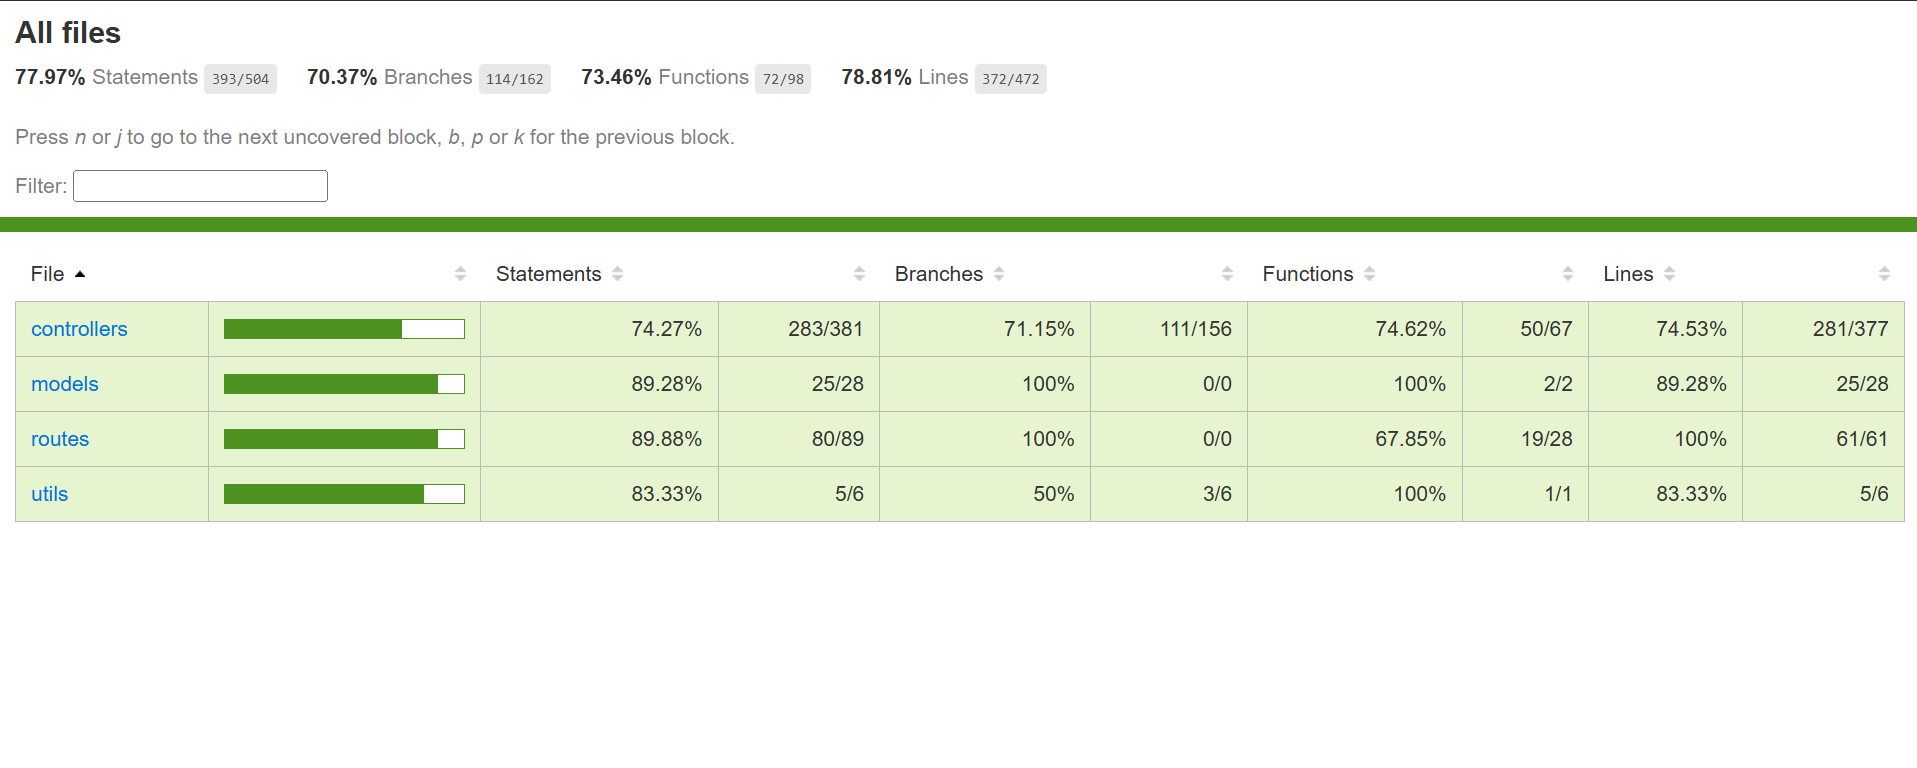
\includegraphics[width=0.9\textwidth]{assets/jest/coverage_test_report_jest.png}
    \caption{Jest Code Coverage Report}
    \label{fig:coverage_report}
\end{figure}

\subsection{Non-Functional Testing}
Non-functional testing evaluates aspects of the system that are not related to specific functions but are critical to user satisfaction and system integrity.

\subsubsection{Performance Testing}
\documentclass[10pt, a4paper]{report}
\usepackage[utf8]{inputenc}
\usepackage{geometry}
\usepackage{longtable}
\usepackage{array} % For better column definitions in longtable
\usepackage{enumitem} % Required for itemize and enumerate options
\usepackage{helvet} % Using a sans-serif font for better readability
\renewcommand{\familydefault}{\sfdefault}

\geometry{left=0.5cm, right=0.5cm, top=2cm, bottom=2cm}

\title{Non-Functional Test Cases: Performance Testing \\ \large Library Management System}
\author{Test Team (Coders \& Non-Coders/Specification Experts)}
\date{June 5, 2025}

\begin{document}
\maketitle
\begin{center}
    \textbf{Note:} These test cases are designed to evaluate the system's performance characteristics, including responsiveness, speed, and stability under various conditions. Metrics are illustrative and should be benchmarked against specific project requirements. Refer to the SRS and Test Plan for complete context.
\end{center}

\section*{IV.C Non-Functional Test Cases: Performance Testing}

\begin{longtable}{|>{\raggedright\arraybackslash}p{3.5cm}|>{\raggedright\arraybackslash}p{4cm}|>{\raggedright\arraybackslash}p{5cm}|>{\raggedright\arraybackslash}p{5.5cm}|}
\caption{Performance Test Cases}\label{tab:perf_test_cases}\\
\hline
\textbf{Test Case ID} & \textbf{Test Title} & \textbf{Test Steps} & \textbf{Expected Results} \\
\hline
\endfirsthead
\multicolumn{4}{c}%
{{\bfseries \tablename\ \thetable{} -- continued from previous page}} \\
\hline
\textbf{Test Case ID} & \textbf{Test Title} & \textbf{Test Steps} & \textbf{Expected Results} \\
\hline
\endhead
\hline \multicolumn{4}{|r|}{{Continued on next page}} \\ \hline
\endfoot
\hline
\endlastfoot

% UI Load & Responsiveness Testing (Non-Coder Focus)
\multicolumn{4}{|l|}{\textbf{Sub-Section: UI Load \& Responsiveness Testing}} \\ \hline
TC\_PERF\_UI\_001 & Page load time for book list with few records & 
    \begin{itemize}[noitemsep, topsep=0pt, partopsep=0pt, leftmargin=*]
        \item \textbf{Precondition:} Database contains a small number of records (e.g., < 50 books).
        \item Login as a Librarian or Member.
        \item Navigate to the book list page ('/books').
        \item Measure the time from navigation start to when the page is fully rendered and interactive.
    \end{itemize} & 
    \begin{itemize}[noitemsep, topsep=0pt, partopsep=0pt, leftmargin=*]
        \item The page load time should be within the acceptable baseline (e.g., < 2 seconds).
        \item The UI is responsive and usable immediately after rendering.
    \end{itemize} \\ \hline
TC\_PERF\_UI\_002 & Page load time for book list with many records (Volume) & 
    \begin{itemize}[noitemsep, topsep=0pt, partopsep=0pt, leftmargin=*]
        \item \textbf{Precondition:} Database contains a large number of records (e.g., > 5,000 books).
        \item Login as a Librarian or Member.
        \item Navigate to the book list page ('/books').
        \item Measure the time until the page is fully rendered and interactive.
    \end{itemize} & 
    \begin{itemize}[noitemsep, topsep=0pt, partopsep=0pt, leftmargin=*]
        \item The page load time meets the defined threshold for large data sets (e.g., < 5 seconds).
        \item UI remains responsive; features like sorting or filtering might show a loading indicator but do not freeze the application.
    \end{itemize} \\ \hline
TC\_PERF\_UI\_003 & UI responsiveness during data entry on a high-load page & 
    \begin{itemize}[noitemsep, topsep=0pt, partopsep=0pt, leftmargin=*]
        \item Navigate to a data-heavy page (e.g., Librarian Dashboard with many widgets).
        \item While the page is rendering or widgets are loading data, attempt to interact with a simple UI element (e.g., open a dropdown menu).
    \end{itemize} & 
    \begin{itemize}[noitemsep, topsep=0pt, partopsep=0pt, leftmargin=*]
        \item User interactions are not blocked.
        \item The UI responds to input within a reasonable time (e.g., < 500ms) without noticeable lag.
    \end{itemize} \\ \hline

% API Response Time Testing (Coder Focus)
\multicolumn{4}{|l|}{\textbf{Sub-Section: API Response Time Testing}} \\ \hline
TC\_PERF\_API\_001 & API response time for fetching all books (Normal Load) & 
    \begin{itemize}[noitemsep, topsep=0pt, partopsep=0pt, leftmargin=*]
        \item \textbf{Precondition:} Database contains a moderate number of book records (e.g., 500).
        \item Using an API testing tool (e.g., Postman), send a GET request to the `/api/book/getAll` endpoint.
        \item Measure the server response time.
    \end{itemize} & 
    \begin{itemize}[noitemsep, topsep=0pt, partopsep=0pt, leftmargin=*]
        \item The API response time is within the defined benchmark (e.g., < 300ms).
        \item The HTTP status code is 200 OK.
    \end{itemize} \\ \hline
TC\_PERF\_API\_002 & API response time for creating a new entity (e.g., Borrowal) & 
    \begin{itemize}[noitemsep, topsep=0pt, partopsep=0pt, leftmargin=*]
        \item Using an API testing tool, send a POST request with a valid payload to the `/api/borrowal/add` endpoint.
        \item Measure the server response time.
    \end{itemize} & 
    \begin{itemize}[noitemsep, topsep=0pt, partopsep=0pt, leftmargin=*]
        \item The API response time for the creation operation is within the benchmark (e.g., < 400ms).
        \item The HTTP status code is 201 Created (or similar success code).
    \end{itemize} \\ \hline
TC\_PERF\_API\_003 & API response time for user authentication & 
    \begin{itemize}[noitemsep, topsep=0pt, partopsep=0pt, leftmargin=*]
        \item Using an API testing tool, send a POST request with valid user credentials to the `/api/auth/login` endpoint.
        \item Measure the server response time.
    \end{itemize} & 
    \begin{itemize}[noitemsep, topsep=0pt, partopsep=0pt, leftmargin=*]
        \item Authentication is a critical path; response time should be fast (e.g., < 250ms).
        \item The HTTP status code is 200 OK.
    \end{itemize} \\ \hline

% Volume Testing
\multicolumn{4}{|l|}{\textbf{Sub-Section: Volume Testing}} \\ \hline
TC\_PERF\_VOL\_001 & System performance with large data volume in multiple tables & 
    \begin{itemize}[noitemsep, topsep=0pt, partopsep=0pt, leftmargin=*]
        \item \textbf{Precondition:} Populate the database with an abnormally large volume of data:
        \begin{itemize}
            \item 20,000+ Books
            \item 5,000+ Users
            \item 50,000+ Borrowal records
        \end{itemize}
        \item Perform a series of common user actions (e.g., login, search for a book, view user list, view borrowal history).
    \end{itemize} & 
    \begin{itemize}[noitemsep, topsep=0pt, partopsep=0pt, leftmargin=*]
        \item The system remains stable and does not crash or become unresponsive.
        \item Data retrieval and display operations complete within defined acceptable limits, though slower than with few records.
        \item Database queries do not time out.
    \end{itemize} \\ \hline

% Stress Testing
\multicolumn{4}{|l|}{\textbf{Sub-Section: Stress Testing}} \\ \hline
TC\_PERF\_STRS\_001 & System stability under high concurrent user load & 
    \begin{itemize}[noitemsep, topsep=0pt, partopsep=0pt, leftmargin=*]
        \item \textbf{Precondition:} Use a load testing tool (e.g., JMeter, Gatling).
        \item Simulate a high number of concurrent users (e.g., 100 users) performing actions simultaneously for a sustained period (e.g., 15 minutes). Actions include:
        \begin{itemize}
            \item Logging in
            \item Fetching book lists
            \item Adding new borrowals
        \end{itemize}
    \end{itemize} & 
    \begin{itemize}[noitemsep, topsep=0pt, partopsep=0pt, leftmargin=*]
        \item The system remains operational and does not crash.
        \item The average API response time degradation is within an acceptable percentage (e.g., does not increase by more than 50% from the baseline).
        \item The error rate (e.g., HTTP 5xx errors) is below a minimal threshold (e.g., < 1%).
    \end{itemize} \\ \hline
TC\_PERF\_STRS\_002 & System recovery after a stress period & 
    \begin{itemize}[noitemsep, topsep=0pt, partopsep=0pt, leftmargin=*]
        \item Following the completion of the TC\_PERF\_STRS\_001 test, stop the load generation.
        \item Wait for a brief period (e.g., 2 minutes).
        \item Perform a single-user check by navigating key pages (Login, Books, Dashboard).
    \end{itemize} & 
    \begin{itemize}[noitemsep, topsep=0pt, partopsep=0pt, leftmargin=*]
        \item The system recovers and returns to normal performance levels.
        \item Response times for the single user should return to the baseline measurements recorded in the API and UI tests.
        \item No data corruption has occurred.
    \end{itemize} \\ \hline

\end{longtable}

\end{document}

\subsubsection{Security Testing}
\begin{longtable}{|>{\scriptsize\raggedright\arraybackslash}p{3cm}|>{\raggedright\arraybackslash}p{3cm}|>{\raggedright\arraybackslash}p{5cm}|>{\raggedright\arraybackslash}p{5cm}|}
\caption{Security Test Cases}\label{tab:security_test_cases}\\
\hline
\textbf{Test Case ID} & \textbf{Test Title} & \textbf{Test Steps} & \textbf{Expected Results} \\
\hline
\endfirsthead
\multicolumn{4}{c}%
{{\bfseries \tablename\ \thetable{} -- continued from previous page}} \\
\hline
\textbf{Test Case ID} & \textbf{Test Title} & \textbf{Test Steps} & \textbf{Expected Results} \\
\hline
\endhead
\hline \multicolumn{4}{|r|}{{Continued on next page}} \\ \hline
\endfoot
\hline
\endlastfoot

% Sub-Section: Access Control & Authorization (RBAC)
\multicolumn{4}{|l|}{\textbf{Sub-Section: Access Control \& Authorization (RBAC)}} \\ \hline
TC\_SEC\_RBAC\_001 & Verify Member cannot access Librarian-only URLs  & 
    \begin{itemize}
        \item Login as a 'Member' user.
        \item Attempt to navigate directly to a Librarian-only URL (e.g., `/users`, `/dashboard`).
    \end{itemize} & 
    \begin{itemize}
        \item Access is denied.
        \item The system redirects the user to an appropriate page (e.g., login page, member dashboard) and does not display the requested admin page.
    \end{itemize} \\ \hline
TC\_SEC\_RBAC\_002 & Verify unauthenticated user cannot access any protected pages  & 
    \begin{itemize}
        \item Ensure no user is logged in (e.g., use a new browser session or clear cookies).
        \item Attempt to navigate directly to any protected URL (e.g., `/books`, `/users`, `/borrowals`).
    \end{itemize} & 
    \begin{itemize}
        \item Access is denied for all protected URLs.
        \item The system redirects the user to the login page.
    \end{itemize} \\ \hline
TC\_SEC\_RBAC\_003 & Member attempts to perform a Librarian action via API  & 
    \begin{itemize}
        \item Login as a 'Member' user and obtain the session token.
        \item Use an API tool (e.g., Postman) to send a request to a Librarian-only API endpoint (e.g., `DELETE /api/user/delete/:id` with a valid user ID).
    \end{itemize} & 
    \begin{itemize}
        \item The API returns an authorization error (e.g., 403 Forbidden or 401 Unauthorized).
        \item The action (e.g., deleting a user) is not performed. The data remains unchanged in the database.
    \end{itemize} \\ \hline

% Sub-Section: Input Validation & Injection Attacks
\multicolumn{4}{|l|}{\textbf{Sub-Section: Input Validation \& Injection Attacks}} \\ \hline
TC\_SEC\_INJ\_001 & Attempt basic Cross-Site Scripting (XSS) in UI form fields  & 
    \begin{itemize}
        \item Login as Librarian.
        \item Navigate to the 'Add Book' form.
        \item In a text field (e.g., 'Summary'), enter a basic XSS payload like \scriptsize\fbox{\texttt{\textless script\textgreater alert('XSS')\textless /script\textgreater}}.
        \item Submit the form to create the book.
        \item View the details of the newly created book.
    \end{itemize} & 
    \begin{itemize}
        \item The script is not executed. No alert box appears.
        \item The input is properly sanitized and displayed as plain text (e.g., \scriptsize\fbox{\texttt{\&lt;script\&gt;alert('XSS')\&lt;/script\&gt;}}) or the input is rejected.
    \end{itemize} \\ \hline
TC\_SEC\_INJ\_002 & Attempt basic NoSQL injection in login form  & 
    \begin{itemize}
        \item Navigate to the login page.
        \item In the email/username field, enter a NoSQL injection payload (e.g., \scriptsize\fbox{\texttt{\{\$ne: null\}}}).
        \item Enter any password and submit.
    \end{itemize} & 
    \begin{itemize}
        \item The login attempt fails.
        \item The system returns a generic error message like \scriptsize\fbox{\texttt{"Invalid username or password"}} and does not crash or reveal system information.
        \item The application is not bypassed.
    \end{itemize} \\ \hline
TC\_SEC\_INJ\_003 & Attempt insecure direct object reference (IDOR) via API  & 
    \begin{itemize}
        \item Login as 'Member A'.
        \item Navigate to 'My Borrowal History' and note the URL or API call used to fetch the data (e.g., `GET /api/borrowal/getAll` which is then filtered by the client ).
        \item Using an API tool, attempt to request details of a specific borrowal that belongs to `Member B' by guessing or obtaining its ID (e.g., `GET /api/borrowal/get/:borrowal\_id\_of\_member\_B`).
    \end{itemize} & 
    \begin{itemize}
        \item The API returns an authorization error (e.g., 403 Forbidden or 404 Not Found).
        \item The details of 'Member B's borrowal record are not displayed.
    \end{itemize} \\ \hline

% Sub-Section: Session Management
\multicolumn{4}{|l|}{\textbf{Sub-Section: Session Management}} \\ \hline
TC\_SEC\_SESS\_001 & Verify session invalidation on logout  & 
    \begin{itemize}
        \item Login as any user.
        \item Copy the URL of a protected page (e.g., `/books`).
        \item Click the 'Logout' button. The user is redirected to the login page.
        \item Click the browser's 'Back' button or paste the copied URL into the address bar.
    \end{itemize} & 
    \begin{itemize}
        \item The protected page is not displayed.
        \item The user remains on the login page or is redirected back to it, confirming the session was terminated.
    \end{itemize} \\ \hline
TC\_SEC\_SESS\_002 & Verify secure session cookie attributes & 
    \begin{itemize}
        \item Login to the application.
        \item Use browser developer tools to inspect the cookies set by the application.
    \end{itemize} & 
    \begin{itemize}
        \item Session cookies should have the `HttpOnly` attribute to prevent access via JavaScript.
        \item Session cookies should have the `Secure` attribute (if using HTTPS) to ensure they are sent only over secure connections.
    \end{itemize} \\ \hline

% Sub-Section: Data Security & Transport Layer
\multicolumn{4}{|l|}{\textbf{Sub-Section: Data Security \& Transport Layer}} \\ \hline
TC\_SEC\_DATA\_001 & Verify sensitive data is not returned in API responses  & 
    \begin{itemize}
        \item Login as Librarian.
        \item Use an API tool to call an endpoint that returns user data (e.g., `GET /api/user/get/:id`).
        \item Inspect the JSON response body.
    \end{itemize} & 
    \begin{itemize}
        \item The response does not contain sensitive data like the user's password hash or salt.
        \item Only necessary and non-sensitive user data is returned (e.g., name, email, role).
    \end{itemize} \\ \hline
TC\_SEC\_DATA\_002 & Verify secure data transmission (HTTPS)  & 
    \begin{itemize}
        \item Access the application in a web browser.
        \item Check the URL in the address bar.
        \item Use browser developer tools to monitor network traffic during login and other operations.
    \end{itemize} & 
    \begin{itemize}
        \item The connection uses HTTPS, indicated by `https://` and a lock icon.
        \item All data, especially login credentials, is sent over the encrypted HTTPS connection.
    \end{itemize} \\ \hline

% Sub-Section: Static Testing
\multicolumn{4}{|l|}{\textbf{Sub-Section: Static Testing (Code Review)}} \\ \hline
TC\_SEC\_STATIC\_001 & Code review for security vulnerabilities  & 
    \begin{itemize}
        \item (Led by Coders) 
        \item Systematically review backend source code, focusing on authentication, session management, and data access logic.
        \item Use a checklist to look for common vulnerabilities (e.g., improper input validation, hardcoded secrets, use of insecure libraries, potential for injection).
        \item Review frontend code for potential XSS vulnerabilities and improper handling of sensitive data.
    \end{itemize} & 
    \begin{itemize}
        \item A report is generated documenting all potential security flaws found in the code.
        \item Vulnerabilities are categorized by severity.
        \item Recommendations for remediation are provided.
    \end{itemize} \\ \hline

\end{longtable}

\subsubsection{Usability Testing}
\begin{longtable}{|p{0.2\textwidth}|p{0.2\textwidth}|p{0.2\textwidth}|p{0.25\textwidth}|p{0.1\textwidth}|}
    \caption{Usability Test Cases} \\
    \hline
    \textbf{Test Case ID} & \textbf{Objective} & \textbf{Test Steps} & \textbf{Expected Results} & \textbf{Status} \\
    \hline
    \endfirsthead
    \multicolumn{5}{c}%
    {{\bfseries \tablename\ \thetable{} -- continued from previous page}} \\
    \hline
    \textbf{Test Case ID} & \textbf{Objective} & \textbf{Test Steps} & \textbf{Expected Results} & \textbf{Status} \\
    \hline
    \endhead
    \hline \multicolumn{5}{|r|}{{Continued on next page}} \\ \hline
    \endfoot
    \hline
    \endlastfoot

    % General Usability
    TC-USAB-001 & Verify the clarity and intuitiveness of the login page. & 1. Navigate to the login page. \newline 2. Observe the layout and labels. \newline 3. Attempt to log in with incorrect credentials. & 1. The page is uncluttered with clear input fields for "Email" and "Password". \newline 2. A clear, non-technical error message is displayed upon failed login. \newline 3. The purpose of the page is immediately understandable. & To Be Executed \\
    \hline
    TC-USAB-002 & Assess the consistency of the main navigation menu across different pages. & 1. Log in as a Librarian. \newline 2. Navigate to Dashboard, Users, Books, and Authors pages. \newline 3. Observe the position, style, and icons of the navigation sidebar. & The navigation sidebar remains in a consistent location and maintains the same look and feel across all pages. The active page is clearly highlighted. & To Be Executed \\
    \hline
    TC-USAB-003 & Evaluate the effectiveness of user feedback for common actions. & 1. Log in as a Librarian. \newline 2. Create a new Author. \newline 3. Update the details of an existing Book. \newline 4. Delete a Genre. & 1. A clear success message (e.g., a toast or snackbar) appears after each successful action. \newline 2. A confirmation dialog appears before the deletion, preventing accidental data loss. \newline 3. Feedback is timely and easy to understand. & To Be Executed \\
    \hline

    % Librarian Specific
    TC-USAB-004 & Evaluate the clarity and usefulness of the Librarian's dashboard. & 1. Log in as a Librarian. \newline 2. View the dashboard. \newline 3. Analyze the widgets for "Total Books", "Total Members", etc. \newline 4. Review the charts. & 1. The dashboard provides a clear, at-a-glance summary of key library statistics. \newline 2. Charts are well-labeled and easy to interpret. \newline 3. The visual hierarchy directs attention to important information. See Figure \ref{fig:dashboard_usability}. & To Be Executed \\
    \hline
    TC-USAB-005 & Test the ease of creating a new user. & 1. Navigate to the "User" page. \newline 2. Click the "New User" button. \newline 3. Fill out the user creation form with valid data. \newline 4. Submit the form. & The process is intuitive. Form fields are clearly labeled, and input requirements (e.g., password complexity) are clear. The new user appears in the user list immediately after creation. & To Be Executed \\
    \hline
    TC-USAB-006 & Test the intuitiveness of the book management workflow. & 1. Navigate to the "Book" page. \newline 2. Use the filter/search bar to find a specific book. \newline 3. Click to edit a book. \newline 4. Change the book's genre and save. & The search functionality is easy to find and use. Editing a book is straightforward, with a clear form and save button. The UI updates instantly to reflect the change. & To Be Executed \\
    \hline

    % Member Specific
    TC-USAB-007 & Evaluate the process of borrowing a book for a Member. & 1. Log in as a Member. \newline 2. Find an available book. \newline 3. Click the "Borrow" button. \newline 4. Confirm the action. & The "Borrow" action is clearly available for books that are not already on loan. The process requires minimal steps. The user receives clear confirmation that the book has been successfully borrowed. & To Be Executed \\
    \hline
    TC-USAB-008 & Assess the clarity of the member's borrowal history page. & 1. Log in as a Member. \newline 2. Navigate to the "Borrowals" page. \newline 3. View the list of current and past borrowals. & The page clearly displays essential information: book title, borrow date, due date, and status (e.g., "Borrowed", "Returned"). The layout is easy to read and understand. See Figure \ref{fig:borrowal_history_usability}. & To Be Executed \\
    \hline
    TC-USAB-009 & Test the ease of leaving a review for a book. & 1. Log in as a Member. \newline 2. Navigate to a book they have borrowed. \newline 3. Find the option to leave a review. \newline 4. Submit a rating and a comment. & The review submission form is easy to find and use. The user can easily select a rating (e.g., via stars) and type a comment. The submitted review appears promptly. & To Be Executed \\
    \hline

\end{longtable}

\begin{figure}[H]
    \centering
    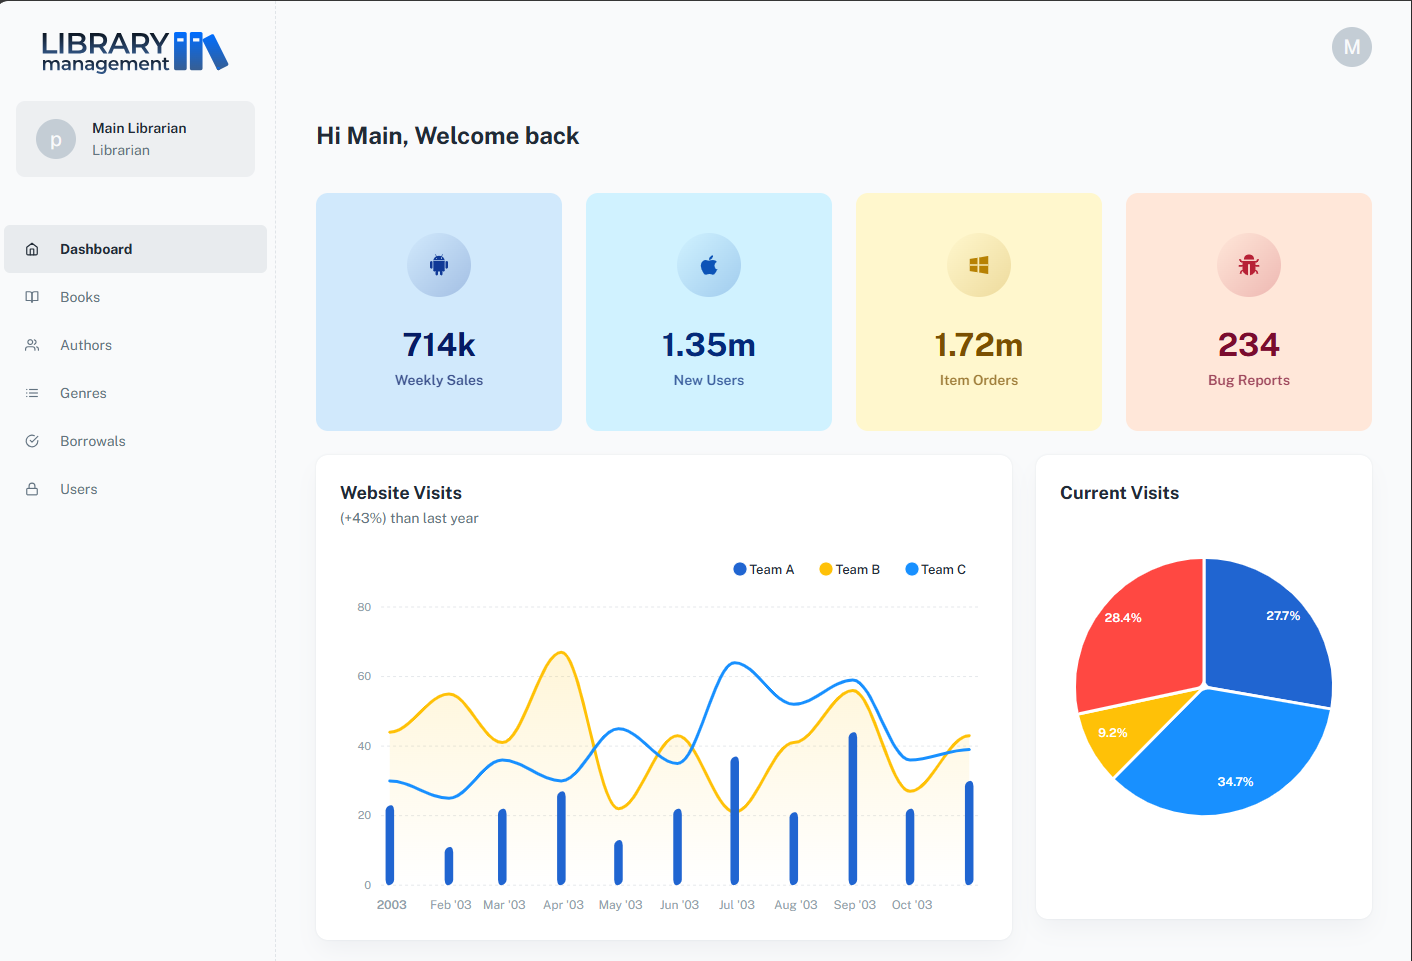
\includegraphics[width=0.9\textwidth]{assets/dashboard_screenshot.png}
    \caption{Librarian Dashboard UI for Usability Evaluation}
    \label{fig:dashboard_usability}
\end{figure}

\begin{figure}[H]
    \centering
    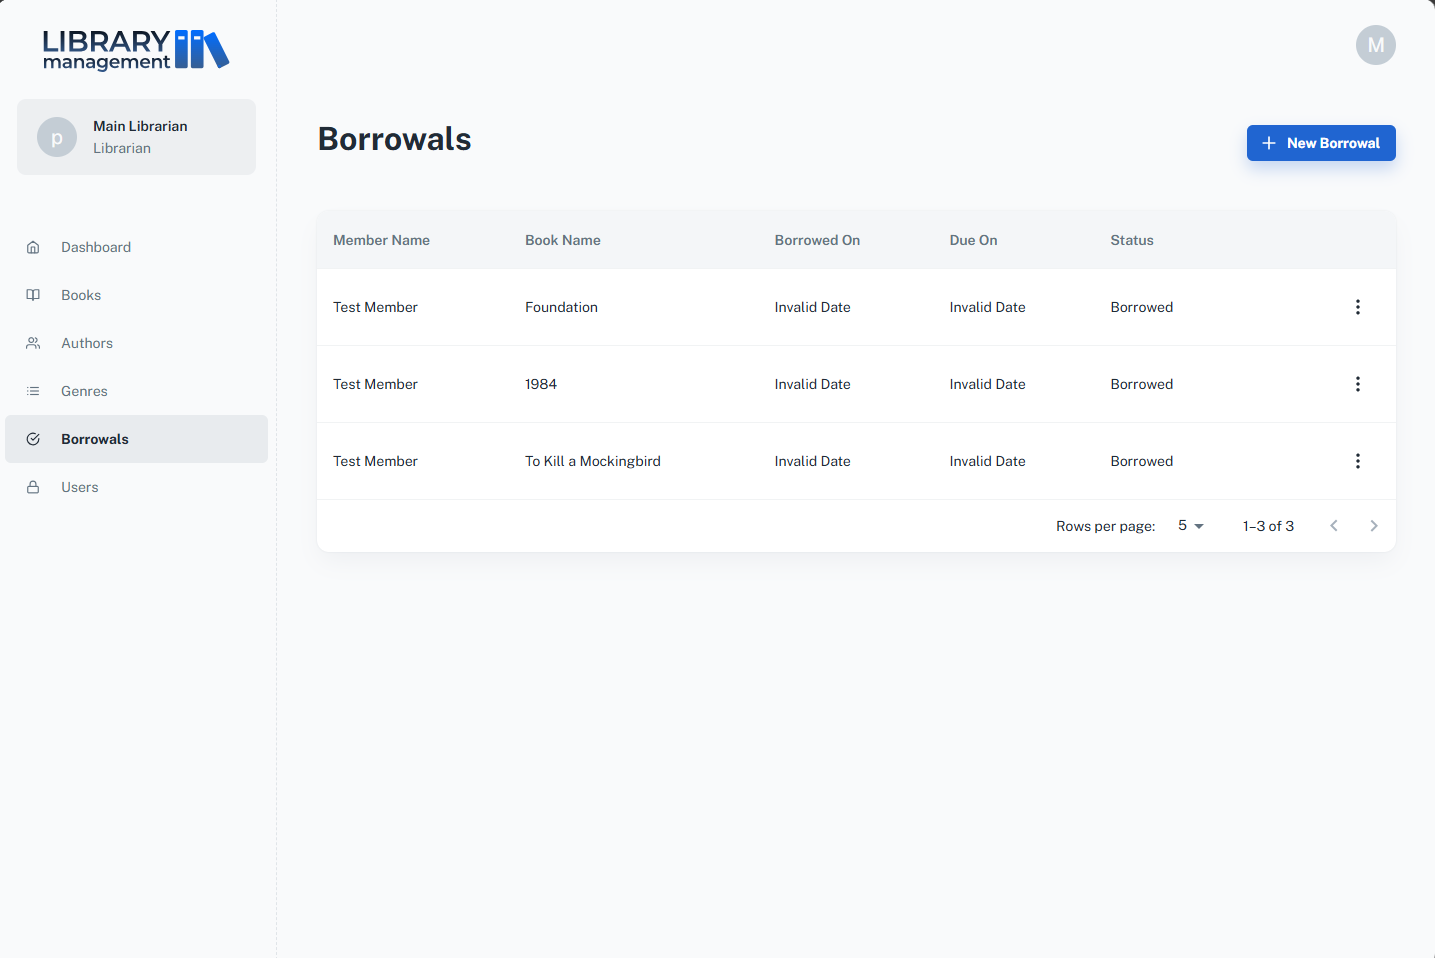
\includegraphics[width=0.9\textwidth]{assets/borrowal_history_member.png}
    \caption{Member Borrowal History UI for Usability Evaluation}
    \label{fig:borrowal_history_usability}
\end{figure}
For a more detailed breakdown of usability heuristics, we utilized a checklist during evaluation:
\input{./test_artifacts/checklists/usability_checklist.tex}

\subsubsection{Browser Compatibility Testing}
\begin{longtable}{|>{\raggedright\arraybackslash}p{3cm}|>{\raggedright\arraybackslash}p{4.5cm}|>{\raggedright\arraybackslash}p{4.5cm}|>{\raggedright\arraybackslash}p{5.5cm}|}
\caption{Browser Compatibility Test Cases}\label{tab:compat_test_cases}\\
\hline
\textbf{Test Case ID} & \textbf{Test Title} & \textbf{Test Steps} & \textbf{Expected Results} \\
\hline
\endfirsthead
\multicolumn{4}{c}%
{{\bfseries \tablename\ \thetable{} -- continued from previous page}} \\
\hline
\textbf{Test Case ID} & \textbf{Test Title} & \textbf{Test Steps} & \textbf{Expected Results} \\
\hline
\endhead
\hline \multicolumn{4}{|r|}{{Continued on next page}} \\ \hline
\endfoot
\hline
\endlastfoot

% Scope Definition
\multicolumn{4}{|p{18cm}|}{\textbf{Testing Scope:} Tests are to be executed on the latest stable versions of the following browsers as specified in the SRS  and testing plan: Google Chrome, Mozilla Firefox, Microsoft Edge, and Safari.} \\ \hline

% General Layout and Responsiveness
\multicolumn{4}{|l|}{\textbf{Sub-Section: General Layout and Core UI Rendering}} \\ \hline
TC\_BC\_GEN\_001 & Verify overall layout and style consistency across browsers & 
    \begin{itemize}[noitemsep, topsep=0pt, partopsep=0pt, leftmargin=*]
        \item Sequentially open each key page (Login, Dashboard, Books, Authors, etc.) on all target browsers.
        \item Visually inspect the overall page layout, including header, footer, sidebar, and main content area.
    \end{itemize} & 
    \begin{itemize}[noitemsep, topsep=0pt, partopsep=0pt, leftmargin=*]
        \item The layout is consistent across all browsers.
        \item All elements are correctly aligned. There are no overlapping or misaligned UI components.
        \item Fonts, colors, and images render correctly and consistently.
        \item No JavaScript errors are present in the developer console.
    \end{itemize} \\ \hline
TC\_BC\_GEN\_002 & Verify responsiveness of the UI on different browser window sizes & 
    \begin{itemize}[noitemsep, topsep=0pt, partopsep=0pt, leftmargin=*]
        \item Open the application on a target browser.
        \item Resize the browser window to simulate different screen sizes (desktop, tablet, mobile).
        \item Observe how the UI elements reflow and adapt.
        \item Repeat for all target browsers.
    \end{itemize} & 
    \begin{itemize}[noitemsep, topsep=0pt, partopsep=0pt, leftmargin=*]
        \item The application remains usable and aesthetically pleasing at all tested sizes.
        \item Navigation and content are accessible.
        \item Responsive design breakpoints behave consistently across all browsers.
    \end{itemize} \\ \hline

% Authentication
\multicolumn{4}{|l|}{\textbf{Sub-Section: Authentication Pages (Login/Logout)}} \\ \hline
TC\_BC\_AUTH\_001 & Verify Login page rendering and functionality & 
    \begin{itemize}[noitemsep, topsep=0pt, partopsep=0pt, leftmargin=*]
        \item Navigate to the Login page on each target browser.
        \item Inspect the rendering of input fields, labels, and the login button.
        \item Enter valid credentials and click "Login".
    \end{itemize} & 
    \begin{itemize}[noitemsep, topsep=0pt, partopsep=0pt, leftmargin=*]
        \item The login form elements are displayed correctly on all browsers.
        \item User is able to type in the fields without issue.
        \item Successful login redirects the user to the correct page, and this behavior is consistent across browsers.
    \end{itemize} \\ \hline
TC\_BC\_AUTH\_002 & Verify error message display on login forms & 
    \begin{itemize}[noitemsep, topsep=0pt, partopsep=0pt, leftmargin=*]
        \item Navigate to the Login page on each target browser.
        \item Attempt to log in with invalid credentials.
        \item Observe the error message.
    \end{itemize} & 
    \begin{itemize}[noitemsep, topsep=0pt, partopsep=0pt, leftmargin=*]
        \item Error messages are displayed clearly and styled correctly on all browsers.
        \item The style and position of the feedback are consistent.
    \end{itemize} \\ \hline

% Core Functionality
\multicolumn{4}{|l|}{\textbf{Sub-Section: Core Functionality (CRUD Operations)}} \\ \hline
TC\_BC\_CRUD\_001 & Verify rendering of data tables/lists & 
    \begin{itemize}[noitemsep, topsep=0pt, partopsep=0pt, leftmargin=*]
        \item As a logged-in Librarian, navigate to a page with a data list (e.g., /books, /users).
        \item Inspect the table's headers, rows, and pagination controls.
        \item Repeat for all target browsers.
    \end{itemize} & 
    \begin{itemize}[noitemsep, topsep=0pt, partopsep=0pt, leftmargin=*]
        \item The data table renders correctly, with proper alignment of columns and rows across all browsers.
        \item Pagination controls are visible, functional, and look the same on all browsers.
    \end{itemize} \\ \hline
TC\_BC\_CRUD\_002 & Verify functionality of forms and dialogs & 
    \begin{itemize}[noitemsep, topsep=0pt, partopsep=0pt, leftmargin=*]
        \item On a management page (e.g., /books), click the "New Book" button to open the creation form/modal.
        \item Inspect all form fields (text inputs, dropdowns, checkboxes).
        \item Trigger a confirmation dialog (e.g., by clicking a "Delete" button).
        \item Repeat for all target browsers.
    \end{itemize} & 
    \begin{itemize}[noitemsep, topsep=0pt, partopsep=0pt, leftmargin=*]
        \item Forms and modals display correctly without any rendering issues across all browsers.
        \item All form controls (text fields, dropdowns, etc.) are fully functional.
        \item Confirmation dialogs appear as expected and are functional on all browsers.
    \end{itemize} \\ \hline
TC\_BC\_CRUD\_003 & Verify client-side form validation & 
    \begin{itemize}[noitemsep, topsep=0pt, partopsep=0pt, leftmargin=*]
        \item Open a creation form (e.g., "Add User").
        \item Submit the form with invalid data (e.g., incorrectly formatted email).
        \item Observe the validation feedback.
        \item Repeat for all target browsers.
    \end{itemize} & 
    \begin{itemize}[noitemsep, topsep=0pt, partopsep=0pt, leftmargin=*]
        \item Client-side validation messages (e.g., "Invalid email format") appear correctly and consistently across all browsers.
        \item The behavior (preventing form submission) is the same on all browsers.
    \end{itemize} \\ \hline

% Specific Features
\multicolumn{4}{|l|}{\textbf{Sub-Section: Feature-Specific Checks}} \\ \hline
TC\_BC\_FEAT\_001 & Verify Librarian Dashboard rendering & 
    \begin{itemize}[noitemsep, topsep=0pt, partopsep=0pt, leftmargin=*]
        \item Login as a Librarian.
        \item Navigate to the Dashboard (/dashboard).
        \item Inspect the layout of statistics widgets and charts.
        \item Repeat for all target browsers.
    \end{itemize} & 
    \begin{itemize}[noitemsep, topsep=0pt, partopsep=0pt, leftmargin=*]
        \item All dashboard widgets and charts are displayed correctly.
        \item The data visualization elements render properly and are legible on all target browsers.
        \item There are no alignment or overlapping issues.
    \end{itemize} \\ \hline
TC\_BC\_FEAT\_002 & Verify JavaScript-driven interactions & 
    \begin{itemize}[noitemsep, topsep=0pt, partopsep=0pt, leftmargin=*]
        \item Interact with UI elements that rely heavily on JavaScript (e.g., filtering a list, sorting a table, using a date picker in a form).
        \item Perform these actions on each target browser.
    \end{itemize} & 
    \begin{itemize}[noitemsep, topsep=0pt, partopsep=0pt, leftmargin=*]
        \item The interactive features work as expected on all browsers.
        \item The performance and behavior of these scripts are consistent.
        \item No browser-specific script errors are logged in the console.
    \end{itemize} \\ \hline

\end{longtable}

\subsection{Regression Testing}
Regression testing is performed to ensure that new code changes, enhancements, or bug fixes do not adversely affect existing functionalities.
\documentclass[10pt, a4paper]{report}
\usepackage[utf8]{inputenc}
\usepackage{geometry}
\usepackage{longtable}
\usepackage{array} % For better column definitions in longtable
\usepackage{enumitem} % Required for itemize and enumerate options
\usepackage{helvet} % Using a sans-serif font for better readability
\renewcommand{\familydefault}{\sfdefault}

\geometry{left=1.5cm, right=1.5cm, top=2cm, bottom=2cm}

\title{VI. Regression Test Suite \\ \large Library Management System}
\author{Test Team}
\date{June 10, 2025}

\begin{document}
\maketitle
\begin{center}
    \textbf{Note:} This regression test suite is designed to verify that recent code changes have not adversely affected existing core functionalities. It focuses on the primary "happy path" scenarios and critical features identified in the SRS. These tests should be executed after every bug fix or feature implementation. 
\end{center}

\section*{VI. Regression Test Cases}

\begin{longtable}{|>{\raggedright\arraybackslash}p{3cm}|>{\raggedright\arraybackslash}p{4cm}|>{\raggedright\arraybackslash}p{5cm}|>{\raggedright\arraybackslash}p{5cm}|}
\caption{Regression Test Suite}\label{tab:regression_test_cases}\\
\hline
\textbf{Test Case ID} & \textbf{Test Title} & \textbf{Test Steps} & \textbf{Expected Results} \\
\hline
\endfirsthead
\multicolumn{4}{c}%
{{\bfseries \tablename\ \thetable{} -- continued from previous page}} \\
\hline
\textbf{Test Case ID} & \textbf{Test Title} & \textbf{Test Steps} & \textbf{Expected Results} \\
\hline
\endhead
\hline \multicolumn{4}{|r|}{{Continued on next page}} \\ \hline
\endfoot
\hline
\endlastfoot

% --- Authentication and Core Access ---
\multicolumn{4}{|l|}{\textbf{Sub-Section: Authentication \& Core Access (Smoke Tests)}} \\ \hline
TC\_REG\_AUTH\_001 & Successful login with valid Librarian credentials & 
    \begin{itemize}[noitemsep, topsep=0pt, partopsep=0pt, leftmargin=*]
        \item Navigate to the login page.
        \item Enter valid Librarian email and password. 
        \item Click the 'Login' button.
    \end{itemize} & 
    \begin{itemize}[noitemsep, topsep=0pt, partopsep=0pt, leftmargin=*]
        \item User is authenticated successfully. 
        \item User is redirected to the Librarian dashboard. 
        \item Librarian-specific functionalities (e.g., 'User Management') are visible. 
    \end{itemize} \\ \hline
TC\_REG\_AUTH\_002 & Successful login with valid Member credentials & 
    \begin{itemize}[noitemsep, topsep=0pt, partopsep=0pt, leftmargin=*]
        \item Navigate to the login page.
        \item Enter valid Member email and password. 
        \item Click the 'Login' button.
    \end{itemize} & 
    \begin{itemize}[noitemsep, topsep=0pt, partopsep=0pt, leftmargin=*]
        \item User is authenticated successfully. 
        \item User is redirected to the books page. 
        \item Librarian-specific functionalities are not visible. 
    \end{itemize} \\ \hline
TC\_REG\_AUTH\_003 & Verify Member cannot access Librarian-specific URLs & 
    \begin{itemize}[noitemsep, topsep=0pt, partopsep=0pt, leftmargin=*]
        \item Login as a Member.
        \item Attempt to navigate directly to the User Management URL (e.g., /users). 
    \end{itemize} & 
    \begin{itemize}[noitemsep, topsep=0pt, partopsep=0pt, leftmargin=*]
        \item Access is denied.
        \item User is redirected to an error page or the member dashboard. 
    \end{itemize} \\ \hline
TC\_REG\_AUTH\_004 & Successful logout for a logged-in user & 
    \begin{itemize}[noitemsep, topsep=0pt, partopsep=0pt, leftmargin=*]
        \item Login as any user (Librarian or Member).
        \item Click the 'Logout' button/link. 
        \item Attempt to use the browser's "back" button to access a protected page.
    \end{itemize} & 
    \begin{itemize}[noitemsep, topsep=0pt, partopsep=0pt, leftmargin=*]
        \item User is logged out successfully and redirected to the login page. 
        \item The user session is terminated, and access to protected pages is denied. 
    \end{itemize} \\ \hline

% --- Core CRUD Functionality (Librarian) ---
\multicolumn{4}{|l|}{\textbf{Sub-Section: Core CRUD Functionality (Librarian)}} \\ \hline
TC\_REG\_CRUD\_001 & Librarian can add a new book & 
    \begin{itemize}[noitemsep, topsep=0pt, partopsep=0pt, leftmargin=*]
        \item Login as Librarian.
        \item Navigate to Book Management (/books). 
        \item Click "New Book" and fill in all required fields (Name, ISBN) with valid, unique data. 
        \item Submit the form.
    \end{itemize} & 
    \begin{itemize}[noitemsep, topsep=0pt, partopsep=0pt, leftmargin=*]
        \item A success message is displayed. 
        \item The new book record is created and appears in the book list. 
    \end{itemize} \\ \hline
TC\_REG\_CRUD\_002 & Librarian can view and update an existing book & 
    \begin{itemize}[noitemsep, topsep=0pt, partopsep=0pt, leftmargin=*]
        \item Login as Librarian and navigate to Book Management.
        \item Select an existing book and choose to edit it.
        \item Change a field (e.g., update the summary).
        \item Save the changes.
    \end{itemize} & 
    \begin{itemize}[noitemsep, topsep=0pt, partopsep=0pt, leftmargin=*]
        \item The book details are displayed correctly in the edit form.
        \item A success message is displayed after saving.
        \item The book list or detail view reflects the updated information.
    \end{itemize} \\ \hline
TC\_REG\_CRUD\_003 & Librarian can register a new user & 
    \begin{itemize}[noitemsep, topsep=0pt, partopsep=0pt, leftmargin=*]
        \item Login as Librarian.
        \item Navigate to User Management (/users). 
        \item Click "New User" and fill in required fields (Name, Email, Password, Role) for a new Member. 
        \item Submit the form.
    \end{itemize} & 
    \begin{itemize}[noitemsep, topsep=0pt, partopsep=0pt, leftmargin=*]
        \item A success message is displayed. 
        \item The new user appears in the user list. 
        \item The newly created user can log in successfully.
    \end{itemize} \\ \hline

% --- Core Use Cases / User Workflows ---
\multicolumn{4}{|l|}{\textbf{Sub-Section: Core Use Cases / User Workflows}} \\ \hline
TC\_REG\_FLOW\_001 & Member can borrow an available book & 
    \begin{itemize}[noitemsep, topsep=0pt, partopsep=0pt, leftmargin=*]
        \item Precondition: A book exists and is marked as available. 
        \item Login as Member.
        \item Navigate to Borrowal Management (/borrowals). 
        \item Click "New Borrowal".
        \item Select the available book. 
        \item Submit the form.
    \end{itemize} & 
    \begin{itemize}[noitemsep, topsep=0pt, partopsep=0pt, leftmargin=*]
        \item A new borrowal record is created successfully with 'Borrowed' status. 
        \item A success message is displayed. 
        \item The availability status of the book is updated to 'false' (unavailable). 
    \end{itemize} \\ \hline
TC\_REG\_FLOW\_002 & Member can view their own borrowal history & 
    \begin{itemize}[noitemsep, topsep=0pt, partopsep=0pt, leftmargin=*]
        \item Precondition: A member has at least one active or past borrowal record.
        \item Login as the Member.
        \item Navigate to the Borrowal Management page (/borrowals). 
    \end{itemize} & 
    \begin{itemize}[noitemsep, topsep=0pt, partopsep=0pt, leftmargin=*]
        \item The page displays a list of borrowal records.
        \item The list contains ONLY the borrowals belonging to the logged-in member. 
    \end{itemize} \\ \hline
TC\_REG\_FLOW\_003 & Librarian can update a borrowal status (e.g., return a book) & 
    \begin{itemize}[noitemsep, topsep=0pt, partopsep=0pt, leftmargin=*]
        \item Precondition: A book has been borrowed by a member.
        \item Login as Librarian.
        \item Navigate to Borrowal Management.
        \item Find the active borrowal record and edit it.
        \item Change the status from 'Borrowed' to 'Returned'. 
        \item Save the changes.
    \end{itemize} & 
    \begin{itemize}[noitemsep, topsep=0pt, partopsep=0pt, leftmargin=*]
        \item The borrowal record's status is successfully updated to 'Returned'.
        \item The corresponding book's availability status is updated back to 'true' (available).
    \end{itemize} \\ \hline

\end{longtable}

\end{document}

\subsection{Installation and Deployment Testing}
This testing ensures that the application can be installed and deployed successfully in the target environments (development, test, production) using the provided Docker configuration.
\begin{longtable}{|p{0.1\textwidth}|p{0.15\textwidth}|p{0.25\textwidth}|p{0.25\textwidth}|p{0.07\textwidth}|p{0.07\textwidth}|}
    \caption{Installation \& Deployment Test Cases}
    \label{tab:installation_tests}\\
    \hline
    \textbf{Test ID} & \textbf{Description} & \textbf{Execution Steps} & \textbf{Expected Results} & \textbf{Status} & \textbf{Notes} \\
    \hline
    \endfirsthead
    \multicolumn{6}{c}%
    {{\bfseries \tablename\ \thetable{} -- continued from previous page}} \\
    \hline
    \textbf{Test ID} & \textbf{Description} & \textbf{Execution Steps} & \textbf{Expected Results} & \textbf{Status} & \textbf{Notes} \\
    \hline
    \endhead
    \hline \multicolumn{6}{|r|}{{Continued on next page}} \\ \hline
    \endfoot
    \hline
    \endlastfoot
    
    TC-IDT-001 & Verify Docker Environment Build and Launch & 
    1. Navigate to the project root directory. \newline
    2. Run the command \texttt{docker-compose up --build -d}. \newline
    3. Check container status with \texttt{docker ps}. & 
    All containers (lms-server, lms-client, lms-db) are running without errors. The client is accessible at \texttt{http://localhost:3000} and the server logs show a successful connection to the database.  & Pass & \\
    \hline
    
    TC-IDT-002 & Verify Database Initialization and Seeding & 
    1. After a fresh launch, connect to the MongoDB container. \newline
    2. Access the \texttt{lms} database. \newline
    3. List collections and query the \texttt{users} collection. & 
    The database contains all required collections as defined by the Mongoose models. The \texttt{users} collection is populated with the initial admin user from the seeding script. & Pass & \\
    \hline
    
    TC-IDT-003 & Post-Deployment Smoke Test (Librarian) & 
    1. Open a browser and navigate to \texttt{http://localhost:3000}. \newline
    2. Log in with Librarian credentials. \newline
    3. Navigate to the Dashboard, Books, and Users pages. & 
    Login is successful. The user is redirected to the Dashboard.  All navigated pages (Dashboard, Books, Users) load correctly without critical errors and display their respective UI components.  & Pass & \\
    \hline
    
    TC-IDT-004 & Post-Deployment Acceptance Test (Member) & 
    1. In a new browser session, log in with Member credentials. \newline
    2. Navigate to the Books page and view a book's details. \newline
    3. Navigate to the Borrowals page to view personal history. & 
    Login is successful. The user is redirected to the Books page.  The user can view the list of books and their details. The borrowal history page loads correctly, displaying a message that no borrowals are found (for a new user).  & Pass & \\
    \hline

    TC-IDT-005 & Verify Docker Build Process & 
    1. Run \texttt{docker-compose build --no-cache} from the root directory. & 
    The Docker images for both the \texttt{server} and \texttt{client} services are built successfully without any errors during dependency installation or code copying.  & Pass & \\
    \hline

    TC-IDT-006 & Verify Graceful Shutdown & 
    1. From the root directory, run the command \texttt{docker-compose down}. \newline
    2. Run \texttt{docker ps -a} to check for remaining containers. & 
    All application containers are stopped and removed. The custom network created by Docker Compose is also removed. No orphaned resources remain. & Pass & \\
    \hline

\end{longtable}

\section{Static Testing}
Static testing is performed without executing the application code. It includes reviews of documentation and source code.
\begin{itemize}
    \item \textbf{Code Reviews:} Manual inspection of source code to identify potential defects, security vulnerabilities, and deviations from coding standards.
    \item \textbf{Walkthroughs:} The development team presents the code to the testing team to explain its logic and flow.
    \item \textbf{Documentation Review:} Review of the SRS, test plan, and other project documents for clarity, completeness, and consistency.
\end{itemize}
\subsubsection{Documentation Review}
All key project documents were subjected to a thorough review process. The review focused on identifying ambiguities, inconsistencies, and missing information. This process ensures that the entire team operates from a shared, unambiguous understanding of the project's goals and specifications.

\begin{itemize}
    \item \textbf{Software Requirements Specification (SRS):} The SRS document was the cornerstone of our review process. It was meticulously examined to ensure that all functional and non-functional requirements were clearly defined, testable, and free from contradiction. Feedback from this review was used to refine the requirements, which in turn guided development and the creation of dynamic test cases.
    \item \textbf{Test Plan and Test Cases:} All documented test cases (including those for functional, API, integration, and non-functional testing) were reviewed to ensure they provided adequate coverage of the requirements. The review verified that test steps were clear, expected outcomes were precise, and traceability to the SRS was established.
    \item \textbf{Tasks and Responsibilities Matrix:} The \texttt{Tasks.tex} document was reviewed to ensure a clear allocation of duties for all testing activities, confirming that every aspect of the test plan had a designated owner.
\end{itemize}

\subsubsection{Code Review and Walkthroughs}
Source code was systematically reviewed to enforce quality and adherence to best practices.

\begin{itemize}
    \item \textbf{Code Reviews:} Peer reviews were conducted for all major components of the application. Developers reviewed each other's code, focusing on logic, efficiency, error handling, security, and compliance with our established coding standards. This process was instrumental in identifying subtle bugs and improving code clarity.
    \item \textbf{Walkthroughs:} For complex workflows, such as the book borrowing and return process, developers conducted walkthroughs. In these sessions, the author of the code explained its structure and logic to other team members, who would ask questions and provide feedback. This method proved highly effective for verifying business logic and ensuring the implementation correctly reflected the use cases defined in the SRS.
\end{itemize}

\subsubsection{Static Testing Test Cases and Findings}
The following table summarizes the key activities performed during static testing and their outcomes. Unlike dynamic tests, these "test cases" represent structured review tasks.

\begin{center}
\begin{longtable}{|p{0.1\textwidth}|p{0.2\textwidth\scriptsize}|p{0.3\textwidth}|p{0.3\textwidth}|}
\caption{Static Testing Cases and Results} \label{tab:static_testing_cases} \\
\hline
\rowcolor{headerColor} \textbf{Test ID} & \textbf{Test Area} & \textbf{Objective} & \textbf{Outcome / Findings} \\
\hline
\endfirsthead
\multicolumn{4}{c}%
{{\bfseries \tablename\ \thetable{} -- continued from previous page}} \\
\hline
\rowcolor{headerColor} \textbf{Test ID} & \textbf{Test Area} & \textbf{Objective} & \textbf{Outcome / Findings} \\
\hline
\endhead
\hline \multicolumn{4}{|r|}{{Continued on next page}} \\ \hline
\endfoot
\hline
\endlastfoot

% --- Documentation Review ---
\textbf{TC-STATIC-001} & SRS Document Review & Verify that all functional requirements are clear, complete, consistent, and testable. & \tick{} The requirements were found to be mostly clear. Minor ambiguities in the book return policy (Use Case UC-003) were identified and clarified with the team. Traceability links to test cases were established. \\
\hline
\textbf{TC-STATIC-002} & Test Plan and Test Cases Review & Ensure comprehensive test coverage for all requirements specified in the SRS. Verify clarity of test steps and expected results. & \tick{} Confirmed that all major use cases were covered by at least one functional or integration test. Some test case descriptions were enhanced for better clarity. \\
\hline
\textbf{TC-STATIC-003} & Tasks \& Responsibilities Review & Confirm that all testing roles and responsibilities are clearly defined and assigned. & \tick{} The roles defined in \texttt{Tasks.tex} were confirmed to be clear and comprehensive, ensuring no gaps in test ownership. \\
\hline

% --- Code Review ---
\textbf{TC-STATIC-004} & Code Review: \texttt{authController.js} & Inspect authentication logic for potential security vulnerabilities (e.g., error message information disclosure) and adherence to best practices. & \tick{} The review identified that initial error messages for failed logins could potentially reveal whether a username exists. The logic was updated to return a generic "Invalid credentials" message in all failure cases. \\
\hline
\textbf{TC-STATIC-005} & Code Review: \texttt{borrowalController.js} & Verify the logic for borrowing, returning, and checking the status of books. Ensure correct state management and handling of edge cases (e.g., borrowing an unavailable book). & \tick{} The core logic was sound. A recommendation was made to add more detailed logging for borrowal transactions to facilitate easier debugging in the future. \\
\hline
\textbf{TC-STATIC-006} & Code Review: Frontend Components (\texttt{/client/src/sections}) & Ensure React components follow best practices for state management, props handling, and separation of concerns. Check for UI consistency. & \tick{} Reviews led to minor refactoring in several components to improve reusability (e.g., creating a generic dialog component). Consistent error handling via \texttt{errorHandler.js} was verified. \\
\hline
\textbf{TC-STATIC-007} & Code Review: Database Models (\texttt{/server/models}) & Review Mongoose schemas for correctness, validation rules, and indexing to ensure data integrity and performance. & \tick{} Confirmed that appropriate validation (e.g., \texttt{required}, \texttt{enum}) was in place. A missing index on the \texttt{email} field of the User model was identified and added to improve query performance. \\
\hline

% --- Walkthrough ---
\textbf{TC-STATIC-008} & Walkthrough: User Registration \& Login Workflow & Walk through the end-to-end code path from the frontend form submission to the backend API, controller logic, and database interaction. & \tick{} The walkthrough confirmed that all team members understood the flow of data and the role of JWT tokens in session management. It clarified the interaction between Passport.js and the custom controller logic. \\
\hline
\textbf{TC-STATIC-009} & Walkthrough: Book Management (CRUD) & Present the code for adding, updating, and deleting books, including referential integrity checks with authors and genres. & \tick{} The walkthrough helped identify a potential race condition if two librarians attempted to delete the same author simultaneously. While a low risk, it highlighted an area for future improvement with more robust transaction management. \\
\hline

\end{longtable}
\end{center}

% It is uncommon to have a dedicated image for static testing results, 
% as they are typically captured in review comments, checklists, or meeting minutes.
% If a visual representation of the review process were needed, a flowchart could be inserted here.
% For example: \includegraphics[width=0.8\textwidth]{assets/static_review_process.png}




\section{Test Environment and Tools}
All testing activities are conducted within a controlled and reproducible environment, managed by Docker. This ensures consistency between development, testing, and production setups.

\begin{longtable}{|p{0.2\textwidth}|p{0.7\textwidth}|}
    \caption{Testing Tools and Frameworks} \\
    \hline
    \textbf{Tool/Framework} & \textbf{Purpose} \\
    \hline
    \endfirsthead
    \multicolumn{2}{c}%
    {{\bfseries \tablename\ \thetable{} -- continued from previous page}} \\
    \hline
    \textbf{Tool/Framework} & \textbf{Purpose} \\
    \hline
    \endhead
    \hline \multicolumn{2}{|r|}{{Continued on next page}} \\ \hline
    \endfoot
    \hline
    \endlastfoot
    Docker & Containerization of the application, database (MongoDB), and testing environments. Used to ensure consistency across all stages. \\
    \hline
    Node.js & The runtime environment for the backend application and test execution. \\
    \hline
    Jest & The primary framework for unit and integration testing of the backend. Provides test running, assertion, and mocking capabilities. \\
    \hline
    Supertest & An HTTP assertion library used with Jest for API integration testing. \\
    \hline
    Cypress & The framework for end-to-end (E2E) system testing, browser compatibility testing, and parts of regression testing. \\
    \hline
    k6 & A modern load testing tool used for performance and stress testing of the API endpoints. \\
    \hline
    MongoDB & The NoSQL database used by the application. A separate test database instance is used for automated testing. \\
    \hline
    Git / GitHub & Version control system for source code and test scripts. Used for collaboration and tracking changes. \\
    \hline
\end{longtable}

\section{Evaluation and Reporting}
The evaluation of the system's quality is a continuous process involving test execution, defect management, and reporting.
\begin{itemize}
    \item \textbf{Test Execution:} Tests are executed automatically via npm scripts (e.g., \texttt{npm test}) and on a continuous integration (CI) server (conceptual).
    \item \textbf{Defect Management:} A systematic approach is used to manage defects. When a test fails, a defect is logged with details including steps to reproduce, severity, and priority. The defect is then assigned, fixed, and re-tested.
    \item \textbf{Test Reporting:} After each test cycle, reports are generated. These include Jest test results (see Figure \ref{fig:jest_report}) and code coverage reports (Figure \ref{fig:coverage_report}). These reports provide a clear overview of the application's health to the entire team.
\end{itemize}

\begin{figure}[H]
    \centering
    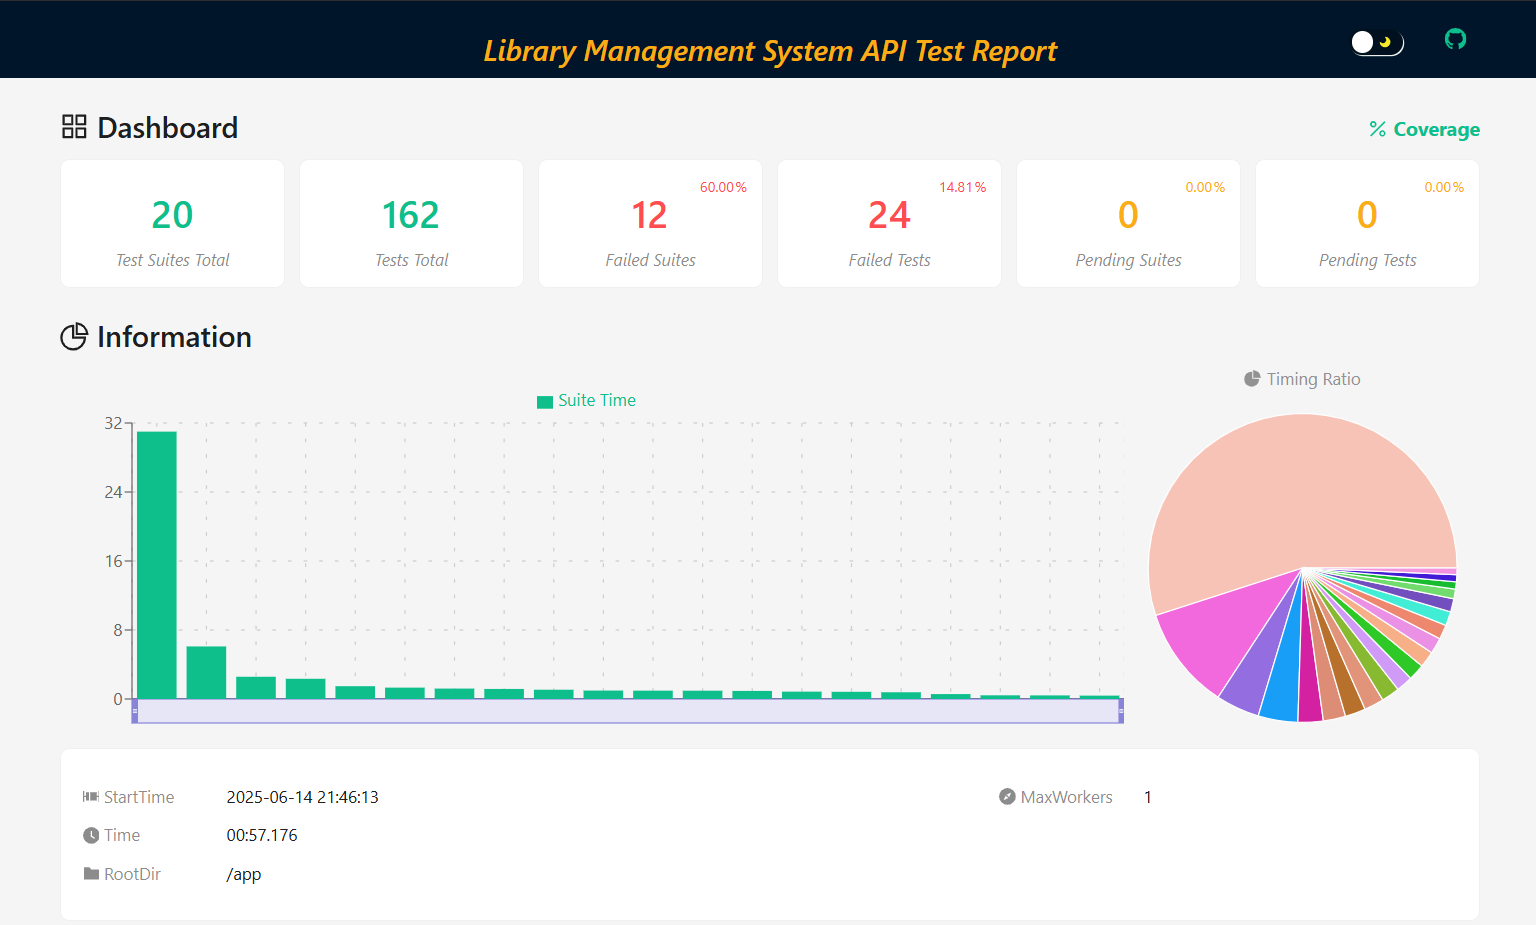
\includegraphics[width=0.9\textwidth]{assets/jest/jest_report_screenshot.png}
    \caption{Jest Test Execution Report}
    \label{fig:jest_report}
\end{figure}

